%\pelliot{To put at the right place}
%\begin{theorem}
%  Let $\Bc=(\Nb, <_\Qb)$ be a dense linear order. Then, there exists a Ramsey enrichment $\hat\Bc$ of $\Bc$. The language $\hat\Lc$ consists of $\Lc$ and an additional relation of arity 4.
%\end{theorem}
%\begin{proof}
%  The predicate $P(a,b,c,d)$ we add to the language will be interpreted as $a\meet b<c\meet d$, for a definition of $\meet$ that we will explain in the proof.
%\end{proof}
%As for every $n$, there is only one embedding type in $\Bc$ of size $n$, in order to know the big Ramsey number for a tuple of $n$ elements, we need to count the number of embedding types in $\hat\Bc$ with $n$ elements.
%\begin{theorem}
%  There are ... Joyce trees with $n$ leaves.
%\end{theorem}
%\begin{corollary}
%  The big Ramsey number for $n$-tuples inside a DLO structure is ...
%\end{corollary}
%\pelliot{End To put at the right place}


%In this subsection, we study the big Ramsey number of the dense linear order.

%\begin{statement}[Devlin's theorem]
 % The statement $\DT{n}{k,\ell}$ is the following: ``for every coloring $f: [\mathbb Q]^n \to k$, there exists a set $S$ order-isomorphic to $\mathbb Q$ such that $[S]^n$ uses at most $\ell$ many colors''.
%\end{statement}
\index{Devlin's theorem}
Devlin's theorem states that the dense linear orders admits big Ramsey numbers, that is, for every $n$ there exists an $\ell$ such that for any finite coloring of the $n$-tuples of rationals, there exists a dense linear subordering of $\Qb$ on which the coloring takes only $\ell$ colors. This corresponds to the statement $(\forall k)\DT{n}{k,\ell}$. Moreover, the function which associates to each $n$ the minimal such $\ell$ is known, being the sequence of the so-called \index{odd tangent numbers} \index{$t_{\DT{}{}}$} ``odd tangent numbers'' $t_{\DT{}{}}(n)$, as defined in \cite[p.~147]{Todorcevic2010Ramsey}. (To list the first few, we have $t_{\DT{}{}}(1) = 1$, $t_{\DT{}{}}(2) = 2$, $t_{\DT{}{}}(3) = 16$, and $t_{\DT{}{}}(4) = 272$.)

%\section{A proof of Devlin's theorem using Milliken's tree theorem}
%
%The link between Devlin's theorem and Milliken's tree theorem is given by the following linear ordering of $\cantor$ in the order type of the rationals:
%
%\begin{definition}[the ordering $<_\Qb$ on $\cantor$]\label{def:leq-Q}
%  Given two strings $\sigma,\tau\in\cantor$, define $\sigma<_\Qb\tau$ if and only if one of the following holds:
%  \begin{enumerate}
%  \item $\sigma\prec\tau$ and $\tau(|\sigma|)=1$
%  \item $\tau\prec\sigma$ and $\sigma(|\tau|)=0$
%  \item $\sigma$ and $\tau$ are incomparable and $\sigma<_{\mathrm{lex}}\tau$, where $<_{\mathrm{lex}}$ is the lexicographical order.
%  \end{enumerate}
%%  \[|\sigma|<|\tau|\land \tau(|\sigma)=1\quad\text{ or }\quad|\tau|<|\sigma|\land \sigma(|\tau)=0\]
%\end{definition}
%Intuitiely, if $\sigma<_\Qb\tau$ then $\sigma$ lies to the left of $\tau$ if one draws the standard picture of the tree $\cantor$, growing upwards from the root. (See, e.g., Figure~\ref{fig:Devlin-to-ACA}.) From this, the claim that this ordering is order-isomorphic to $\Qb$ is clear. An explicit embedding of $<_\Qb$ into $\Qb$ is given by the following function: $\sigma\mapsto\sum_{i<|\sigma|}(\sigma(i)-\frac12)2^{-i}$. Thus, the $i$th bit of $\sigma$ contributes to the sum either $-2^{-i-1}$ or $2^{-i-1}$, depending as it is $0$ or $1$.
%
%Using order $<_\Qb$, we can now prove Devlin's theorem from Milliken's tree theorem, as follows.
%
%\begin{theorem}
%  For every $n$, $\MT{2n-1}{}$ proves $\DT{n}{<\infty,t_{\DT{}{}}(n)}$.
%\end{theorem}
%\begin{proof}
%  Let $f:[\Qb]^n\to k$ be a coloring. As $(\Qb,<)\cong(\cantor,<_\Qb)$, this yields a $k$-coloring of the $n$-tuples of $\cantor$. Recall from Lemma~\ref{lem:tuple-to-height} that $n$ strings generate a strong tree of at most height $2n-1$. We can thus apply $\MT{2n-1}{}$ to $f$ to obtain a strong subtree $S$ such that all representatives of each of these $t_{\DT{}{}}(n)$ many embedding types have the same color. We can then use the construction from \cite[Lemma 6.20]{Todorcevic2010Ramsey} to get a subset $S'\subseteq S$ which is
%  %the $n$-tuples of strings from $S'$ generate at most $t_{\DT{}{}}(n)$ embedding types, and such that $S'$ is
%  a dense linear ordering without endpoints under $<_\Qb$.
%  %The full details of the construction can be found in \cite[Lemma 6.20]{Todorcevic2010Ramsey}, but
%  (In gist, the construction proceeds by building a perfect tree with no nodes at the same level, extending to the left whenever possible, and leaving space between levels. Then, ``blossom'' elements are added above each node in the remaining levels, which are all pairwise incompatible. The blossoms form the desired set $S'$. A helpful picture can be found in \cite[Figure 6.5]{Todorcevic2010Ramsey}. Note that $S'$ is not even a tree.)
%\end{proof}

\section{A big Ramsey structure for dense linear orders}

As explained before, the big Ramsey degree of Devlin's theorem for pairs is 2, while there is only one sub-order of size 2. We now describe an enrichment to the language of orders to
obtain a big Ramsey structure, in the sense of \Cref{def:big-ramsey-structure}, of the dense linear orders with no endpoints.

We will see that we can represent any countable order as an anti-chain $A$ in $\cantor$ with respect to the prefix relation, equipped with the lexicographic order $\ltlex$. \index{$\ltlex$}\index{ordering!$\ltlex$} Then, given two elements $\sigma, \tau \in A$, some extra structure induced by the string representation can be exploited, such as the comparison between the length of $\sigma$ and the length of $\tau$, but as well with respect to length of their meet $\sigma \meet \tau$. 

%\peter{The defn of meet closure in section 7 needs to be moved much earlier.  I used this in the paragraph above.}\ludovic{I removed the meet-closure from the paragraph above since it should really be $A$, not $A^\wedge$.}

As we will see in \Cref{thm:joyce-orders-can-be-coded} we can always ensure that the length of any string in $A^\wedge = \{ \sigma \meet \tau: \sigma, \tau \in A \}$ is unique\index{$A^\wedge$}. There are then 2 possible cases for a pair  $\sigma \ltlex \tau$ in $A$: either $|\sigma| >_\Nb |\tau|$, or $|\sigma| <_\Nb |\tau|$. The case of the equality has been ruled out since all lengths of the strings in $A^\wedge$ will be unique. While there are examples where their lengths are not unique (see the figure below), the example where they are unique will prove to be very illustrative. 

A finite subset of $n$ elements in $A$ can be represented as a particular kind of binary tree, known as a Joyce tree. A \emph{Joyce tree} \index{Joyce!tree}\index{tree!Joyce}of size $n$ is a labeled tree with $2n-1$ vertices, such that every non-leaf has exactly two immediate children. The labels \index{label!Joyce tree} are among $\{1, \dots, 2n-1\}$ and so that every child has a label greater than its parent (see Street~\cite{streets}). See \Cref{fig:joyce-trees} for some examples of Joyce trees.

\begin{figure}[htbp]
\centering
%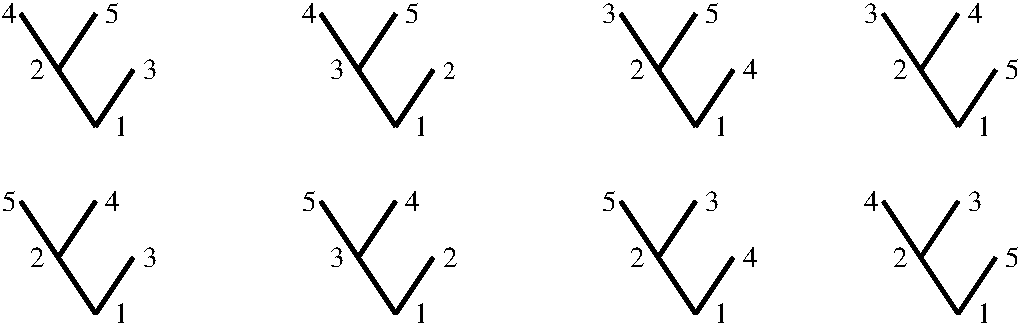
\includegraphics[scale=0.6]{figures/balJoyceTrees.pdf}
% \includegraphics[width=10cm]{drawings/joyce-trees.jpg}
	\begin{tikzpicture}[scale=1.5,font=\normalsize]
		\tikzset{
			empty node/.style={circle,inner sep=0,fill=none},
			solid node/.style={circle,draw,inner sep=1.5,fill=black},
			hollow node/.style={circle,draw,inner sep=1.5,fill=white},
			gray node/.style={circle,draw={rgb:black,1;white,4},inner sep=1.5,fill={rgb:black,1;white,4}}
		}
		\tikzset{snake it/.style={decorate, decoration=snake, line cap=round}}
		\tikzset{gray line/.style={line cap=round,thick,color={rgb:black,1;white,4}}}
		\tikzset{thick line/.style={line cap=round,rounded corners=0.1mm,thick}}
		\node (a)[empty node,label=below:{$1$}] at (0,0) {};
		\node (b)[empty node,label=below:{$2$}] at (-0.4,0.5) {};
		\node (c)[empty node,label=above:{$3$}] at (0.4,0.5) {};
		\node (d)[empty node,label=above:{$4$}] at (-0.8,1) {};
		\node (e)[empty node,label=above:{$5$}] at (0,1) {};
		\draw[thick line] (a.center) to (b.center) to (d.center);
		\draw[thick line] (b.center) to (e.center);
		\draw[thick line] (a.center) to (c.center);
	\end{tikzpicture}
	\hspace{5mm}
	\begin{tikzpicture}[scale=1.5,font=\normalsize]
		\tikzset{
			empty node/.style={circle,inner sep=0,fill=none},
			solid node/.style={circle,draw,inner sep=1.5,fill=black},
			hollow node/.style={circle,draw,inner sep=1.5,fill=white},
			gray node/.style={circle,draw={rgb:black,1;white,4},inner sep=1.5,fill={rgb:black,1;white,4}}
		}
		\tikzset{snake it/.style={decorate, decoration=snake, line cap=round}}
		\tikzset{gray line/.style={line cap=round,thick,color={rgb:black,1;white,4}}}
		\tikzset{thick line/.style={line cap=round,rounded corners=0.1mm,thick}}
		\node (a)[empty node,label=below:{$1$}] at (0,0) {};
		\node (b)[empty node,label=below:{$3$}] at (-0.4,0.5) {};
		\node (c)[empty node,label=above:{$2$}] at (0.4,0.5) {};
		\node (d)[empty node,label=above:{$4$}] at (-0.8,1) {};
		\node (e)[empty node,label=above:{$5$}] at (0,1) {};
		\draw[thick line] (a.center) to (b.center) to (d.center);
		\draw[thick line] (b.center) to (e.center);
		\draw[thick line] (a.center) to (c.center);
	\end{tikzpicture}
	\hspace{5mm}
	\begin{tikzpicture}[scale=1.5,font=\normalsize]
		\tikzset{
			empty node/.style={circle,inner sep=0,fill=none},
			solid node/.style={circle,draw,inner sep=1.5,fill=black},
			hollow node/.style={circle,draw,inner sep=1.5,fill=white},
			gray node/.style={circle,draw={rgb:black,1;white,4},inner sep=1.5,fill={rgb:black,1;white,4}}
		}
		\tikzset{snake it/.style={decorate, decoration=snake, line cap=round}}
		\tikzset{gray line/.style={line cap=round,thick,color={rgb:black,1;white,4}}}
		\tikzset{thick line/.style={line cap=round,rounded corners=0.1mm,thick}}
		\node (a)[empty node,label=below:{$1$}] at (0,0) {};
		\node (b)[empty node,label=below:{$2$}] at (-0.4,0.5) {};
		\node (c)[empty node,label=above:{$4$}] at (0.4,0.5) {};
		\node (d)[empty node,label=above:{$3$}] at (-0.8,1) {};
		\node (e)[empty node,label=above:{$5$}] at (0,1) {};
		\draw[thick line] (a.center) to (b.center) to (d.center);
		\draw[thick line] (b.center) to (e.center);
		\draw[thick line] (a.center) to (c.center);
	\end{tikzpicture}
	\hspace{5mm}
	\begin{tikzpicture}[scale=1.5,font=\normalsize]
		\tikzset{
			empty node/.style={circle,inner sep=0,fill=none},
			solid node/.style={circle,draw,inner sep=1.5,fill=black},
			hollow node/.style={circle,draw,inner sep=1.5,fill=white},
			gray node/.style={circle,draw={rgb:black,1;white,4},inner sep=1.5,fill={rgb:black,1;white,4}}
		}
		\tikzset{snake it/.style={decorate, decoration=snake, line cap=round}}
		\tikzset{gray line/.style={line cap=round,thick,color={rgb:black,1;white,4}}}
		\tikzset{thick line/.style={line cap=round,rounded corners=0.1mm,thick}}
		\node (a)[empty node,label=below:{$1$}] at (0,0) {};
		\node (b)[empty node,label=below:{$2$}] at (-0.4,0.5) {};
		\node (c)[empty node,label=above:{$5$}] at (0.4,0.5) {};
		\node (d)[empty node,label=above:{$3$}] at (-0.8,1) {};
		\node (e)[empty node,label=above:{$4$}] at (0,1) {};
		\draw[thick line] (a.center) to (b.center) to (d.center);
		\draw[thick line] (b.center) to (e.center);
		\draw[thick line] (a.center) to (c.center);
	\end{tikzpicture}\\
	\medskip
	\begin{tikzpicture}[scale=1.5,font=\normalsize]
		\tikzset{
			empty node/.style={circle,inner sep=0,fill=none},
			solid node/.style={circle,draw,inner sep=1.5,fill=black},
			hollow node/.style={circle,draw,inner sep=1.5,fill=white},
			gray node/.style={circle,draw={rgb:black,1;white,4},inner sep=1.5,fill={rgb:black,1;white,4}}
		}
		\tikzset{snake it/.style={decorate, decoration=snake, line cap=round}}
		\tikzset{gray line/.style={line cap=round,thick,color={rgb:black,1;white,4}}}
		\tikzset{thick line/.style={line cap=round,rounded corners=0.1mm,thick}}
		\node (a)[empty node,label=below:{$1$}] at (0,0) {};
		\node (b)[empty node,label=below:{$2$}] at (-0.4,0.5) {};
		\node (c)[empty node,label=above:{$3$}] at (0.4,0.5) {};
		\node (d)[empty node,label=above:{$5$}] at (-0.8,1) {};
		\node (e)[empty node,label=above:{$4$}] at (0,1) {};
		\draw[thick line] (a.center) to (b.center) to (d.center);
		\draw[thick line] (b.center) to (e.center);
		\draw[thick line] (a.center) to (c.center);
	\end{tikzpicture}
	\hspace{5mm}
	\begin{tikzpicture}[scale=1.5,font=\normalsize]
		\tikzset{
			empty node/.style={circle,inner sep=0,fill=none},
			solid node/.style={circle,draw,inner sep=1.5,fill=black},
			hollow node/.style={circle,draw,inner sep=1.5,fill=white},
			gray node/.style={circle,draw={rgb:black,1;white,4},inner sep=1.5,fill={rgb:black,1;white,4}}
		}
		\tikzset{snake it/.style={decorate, decoration=snake, line cap=round}}
		\tikzset{gray line/.style={line cap=round,thick,color={rgb:black,1;white,4}}}
		\tikzset{thick line/.style={line cap=round,rounded corners=0.1mm,thick}}
		\node (a)[empty node,label=below:{$1$}] at (0,0) {};
		\node (b)[empty node,label=below:{$3$}] at (-0.4,0.5) {};
		\node (c)[empty node,label=above:{$2$}] at (0.4,0.5) {};
		\node (d)[empty node,label=above:{$5$}] at (-0.8,1) {};
		\node (e)[empty node,label=above:{$4$}] at (0,1) {};
		\draw[thick line] (a.center) to (b.center) to (d.center);
		\draw[thick line] (b.center) to (e.center);
		\draw[thick line] (a.center) to (c.center);
	\end{tikzpicture}
	\hspace{5mm}
	\begin{tikzpicture}[scale=1.5,font=\normalsize]
		\tikzset{
			empty node/.style={circle,inner sep=0,fill=none},
			solid node/.style={circle,draw,inner sep=1.5,fill=black},
			hollow node/.style={circle,draw,inner sep=1.5,fill=white},
			gray node/.style={circle,draw={rgb:black,1;white,4},inner sep=1.5,fill={rgb:black,1;white,4}}
		}
		\tikzset{snake it/.style={decorate, decoration=snake, line cap=round}}
		\tikzset{gray line/.style={line cap=round,thick,color={rgb:black,1;white,4}}}
		\tikzset{thick line/.style={line cap=round,rounded corners=0.1mm,thick}}
		\node (a)[empty node,label=below:{$1$}] at (0,0) {};
		\node (b)[empty node,label=below:{$2$}] at (-0.4,0.5) {};
		\node (c)[empty node,label=above:{$4$}] at (0.4,0.5) {};
		\node (d)[empty node,label=above:{$5$}] at (-0.8,1) {};
		\node (e)[empty node,label=above:{$3$}] at (0,1) {};
		\draw[thick line] (a.center) to (b.center) to (d.center);
		\draw[thick line] (b.center) to (e.center);
		\draw[thick line] (a.center) to (c.center);
	\end{tikzpicture}
	\hspace{5mm}
	\begin{tikzpicture}[scale=1.5,font=\normalsize]
		\tikzset{
			empty node/.style={circle,inner sep=0,fill=none},
			solid node/.style={circle,draw,inner sep=1.5,fill=black},
			hollow node/.style={circle,draw,inner sep=1.5,fill=white},
			gray node/.style={circle,draw={rgb:black,1;white,4},inner sep=1.5,fill={rgb:black,1;white,4}}
		}
		\tikzset{snake it/.style={decorate, decoration=snake, line cap=round}}
		\tikzset{gray line/.style={line cap=round,thick,color={rgb:black,1;white,4}}}
		\tikzset{thick line/.style={line cap=round,rounded corners=0.1mm,thick}}
		\node (a)[empty node,label=below:{$1$}] at (0,0) {};
		\node (b)[empty node,label=below:{$2$}] at (-0.4,0.5) {};
		\node (c)[empty node,label=above:{$5$}] at (0.4,0.5) {};
		\node (d)[empty node,label=above:{$4$}] at (-0.8,1) {};
		\node (e)[empty node,label=above:{$3$}] at (0,1) {};
		\draw[thick line] (a.center) to (b.center) to (d.center);
		\draw[thick line] (b.center) to (e.center);
		\draw[thick line] (a.center) to (c.center);
	\end{tikzpicture}
\caption{Eight Joyce trees among the sixteen Joyce trees with three leaves. The eight remaining Joyce trees are mirror reflections of these along a vertical axis though the root node.}
\label{fig:joyce-trees}
\end{figure}

%The labels of the leaves of a Joyce tree correspond to the length of the elements of $A$, while the labels of the branching nodes correspond of the length of their meets.  %% not true in our example. 

Recall that a function is \emph{symmetric} \index{function!symmetric}if its value is the same no matter the order of its arguments. In what follows, we use the string representation of a countable order $(X, <)$ to enriching the order with a symmetric relation binary function $\meetlevel{\cdot}{\cdot}: X^2\to \Nb$.   We shall later refer to any value of the range of $\meetlevel{\cdot}{\cdot}$ as a \emph{label}. \index{label!Joyce order}  %One can think of a label $\meetlevel{x}{y}$ as the length of the longest common substring of $x$ and $y$, given a string representation of $x$ and $y$. 
The label of an element $x \in X$ is $\meetlevel{x}{x}$ and $\meetlevel{x}{y}$ is the label given to $x \meet y$. Again the illustrative example is when all lengths are unique, is to consider the lengths of these nodes as the labels.  

However there are other examples. Consider the first tree in \Cref{fig:joyce-trees} and name its leaves $x$, $y$ and $z$, from left to right. This tree induces a symmetric function $\meetlevel{\cdot}{\cdot}: \{x, y, z\}^2 \to \{1, \dots, 5\}$ as follows: $\meetlevel{x}{x} = 4$, $\meetlevel{y}{y} = 5$, $\meetlevel{z}{z} = 3$, $\meetlevel{x}{y} = 2$, $\meetlevel{x}{z} = 1$, $\meetlevel{y}{z} = 1$. The tree representation also induces an ordering of the labels $\{1, \dots, 5\}$ by reading them from left to right. In this case, $4 < 2 < 5 < 1 < 3$. As we will later see in \Cref{JOtoJT}  $(\{x, y, z\}, <, \meetlevel{\cdot}{\cdot})$ can be used to recover the original Joyce tree. 



%This yields the notion of Joyce order, which can be thought of the set of leaves of a Joyce tree.
%There exists exactly two Joyce orders of length 2, each of which admits big Ramsey degree 1.
%Joyce orders make explicit the hidden underlying structure of dense linear orders with respect to the Ramsey property.
%


\begin{definition}\label{def:jo}\index{$\meetlevel{\cdot}{\cdot}$}\index{order!Joyce}\index{Joyce!order}
  A \emph{Joyce order} is an order $(X,<)$ equipped with a symmetric function $\meetlevel{\cdot}{\cdot}: X^2\to \Nb$ such that for every $x, y, z, t\in X$, not all equal, with $x\leq y$ and $z\leq t$:
  \begin{enumerate}
  \item[\Jo{1}] $\meetlevel{x}{y} <_\Nb \meetlevel{x}{z}\implies(x< y\iff z< y)$;
  \item[\Jo{2}] $\meetlevel{x}{y}<_\Nb\meetlevel{x}{z}\implies\meetlevel{x}{y} = \meetlevel{z}{y}$;
  \item[\Jo{3}] $\meetlevel{x}{y}=\meetlevel{z}{t}\implies \meetlevel{x}{y}<_\Nb\min(\meetlevel{x}{z}, \meetlevel{y}{t})$.
  \end{enumerate}
\end{definition}

Note that the axioms of a Joyce order are universal, hence every subset of a Joyce order induces again a Joyce order.

%\peter{I am still confused by the paragraph after 5.1.  Could you first explain what [[ ]] is for some of the Joyce trees in figure 5.  I would like to 
%semantically understand a JS.   Maybe move def 5.5 to right after 5.1 and then explain the JS for the JO in figure 5.  Please write out that 5.2 1. says the label of meet is less than the label of x and y 2. Says all leafs have unique labels, 3 says that all leafs are not meets.  Maybe you want to have this lemma before you have the paragraph after 5.1 which tries to give an intuition to these rules.}

%%One can think of a Joyce order as the set of leaves of a binary tree whose meets have unique label.
% One can think of a label $\ell = \meetlevel{x}{y}$ as the length of the longest common substring of $x$ and $y$, given a string representation of $x$ and $y$. The label of an element $x \in X$ is $\meetlevel{x}{x}$. Following the previous intuition, $\meetlevel{x}{x}$ corresponds to the length of the string representation of $x$. 

Every Joyce tree gives rise to a Joyce order. Let $X$ be the set of leaves, $\meetlevel{x}{y}$ be the label of the node $x \meet y$, and $\ltlex$ be the lexicographical order on $X$. Then, we claim that $(X,\ltlex,\meetlevel\cdot\cdot)$ is a Joyce order: If $\meetlevel x y<_\Nb\meetlevel x z$, then as $x\meet y$ and $x\meet z$ are comparable and every child has a label greater than its parent, $x\meet y\prec x\meet z$. But then, $x\ltlex y\iff (x\meet z)\ltlex y\iff z\ltlex y$, and $x\meet y = (x\meet z)\meet y=z\meet y$, so both \Jo1 and \Jo2 hold. Finally let $x,y,z,t\in X$ not all equal be such that $\meetlevel xy=\meetlevel zt$. By injectivity of the labelling, $x\meet y= z\meet t$. If $x=y$ then $x\meet y =x$ is a leaf, so $z\meet t$ is a leaf, thus $x=y=z=t$, a contradiction. Therefore, $x\neq y$ and $z\neq t$. Now, suppose $y=z$. As a Joyce tree is binary branching, and $x\ltlex y=z\ltlex t$, one cannot have $x\meet y=z\meet t$, a contradiction. Finally suppose that $x,y,z,t$ are all different. The fact that $x\ltlex y$ and $z\ltlex t$ implies $(x\meet y)0\preceq x$ and $(x\meet y)0\preceq z$, so $x\meet y\prec x\meet z$. By the fact that the label of a child is greater than those of its parents, $\meetlevel xy<_\Nb\meetlevel xz$. Similarly, $\meetlevel xy<_\Nb\meetlevel yt$.  %\peter{I will let someone else finish this proof.  We need this since we are counting finite JO, JT and JS of size n as the same.  This is now mentioned after Lemma 5.6.}

We can use the illustrative example when $X \subseteq \omega^{<\omega}$, $<$ is $<_{lex}$, and all lengths in $X^\wedge = \{\sigma \meet \tau: \sigma, \tau \in X \}$ are unique to get an intuition into these rules. Assume $x\meet z$ is longer than $x\meet y$.  \Jo{1} says that either $y$ is to the left  of both $x$ and $z$ (i.e. $y< x$ and $y < z$) or $y$ is to the right of both $x$ and $z$. \Jo{2} says that $x\meet y = z \meet y $ (after all $x \meet y \preceq x \meet z$). 
%The axiom \Jo{1} informally states that if $z$ and $x$ belong to the same branch but $y$ does not, then $y$ must be either on the left or on the right of both elements. Therefore, it asserts that the order has to be compatible with the tree structure. In particular, one can refer to the order to decide whether $x$ belongs to the left or right branch after a meet. The second axiom \Jo{2} is similar to the first one, but for meets: it basically says that the meets have to be compatible with the tree structure.
The third axiom \Jo{3} says that if both pairs $x, y$ and $z, t$ have a meet with the same label, $x< y$, and $z < t$, then $x \meet z$ must properly above $x \meet y$ and similarly for $y \meet t$.  This implies the meets are binary branching in $X^\wedge$. This also implies that different meets must have different labels. 




%The following lemma states some essential properties of Joyce orders.

\begin{lemma}\label{lem:prop-of-JO}
  The following is true in any Joyce order $(X,<,\meetlevel{\cdot}{\cdot})$:
  \begin{enumerate}
  \item\label{it:prop-of-JO-0} for all $x,y \in X$ with $x\neq y$, $\meetlevel{x}{y} <_\Nb \min(\meetlevel{x}{x}, \meetlevel{y}{y})$;
  \item\label{it:prop-of-JO-1} for all $x,y \in X$ with $x\neq z$, $\meetlevel{x}{x}\neq \meetlevel{z}{z}$;
  \item\label{it:prop-of-JO-2} for all $x,z,t \in X$ with $z\neq t$, $\meetlevel{x}{x}\neq \meetlevel{z}{t}$.
%  \item\label{it:prop-of-JO-3} $\forall x,z,t\in X$ not all equal, $\lnot(\meetlevel{x}{z}= \meetlevel{z}{t}= \meetlevel{x}{t})$.
%  \item\label{it:prop-of-JO-3} $\forall x,y,t\in X$ with $x\neq y$, $|x\meet y|=|\neq |z\meet t|$.
  \end{enumerate}
\end{lemma}
\begin{proof}
  Item 1: by \Jo{3} with $x=z$ and $y=t$.
  Item 2: by \Jo{3} with $x=y$ and $z=t$, $\meetlevel{x}{x}=\meetlevel{z}{z}\implies \meetlevel{x}{x}<_\Nb\min(\meetlevel{x}{z}, \meetlevel{x}{z})$. By Item 1, $\meetlevel{x}{x}<_\Nb\min(\meetlevel{x}{z}, \meetlevel{x}{z})$ cannot hold, so $\meetlevel{x}{x}\neq\meetlevel{z}{z}$.
  Item 3: by \Jo{3} with $x=y$, $\meetlevel{x}{x}=\meetlevel{z}{t}\implies \meetlevel{x}{x}<_\Nb\min(\meetlevel{x}{z}, \meetlevel{x}{t})$. Since $z \neq t$, then either $x \neq z$ or $x \neq t$. In either case, by Item 1, $\meetlevel{x}{z} <_\Nb \meetlevel{x}{x}$ or $\meetlevel{x}{t} <_\Nb \meetlevel{x}{x}$, so $\meetlevel{x}{x}<_\Nb\min(\meetlevel{x}{z}, \meetlevel{x}{t})$ cannot hold, hence $\meetlevel{x}{x}\neq\meetlevel{z}{t}$.

%  Item 4: The case where two elements are equal is already tackled by item 3 \Jo{3} with $x=z$ and $y=t$. Otherwise, suppose without loss of generality that $x<z<t$, then the result follow by \Jo3 with $y=z$.
\end{proof}
% \begin{lemma}\label{lem:size-of-Joyce-order}
%   Let $(F,<,\meetlevel\cdot\cdot)$ be a Joyce order with $|F|=n$. Then, the range $\{\meetlevel ab:a,b\in F\}$ is of cardinality $2n-1$.
% \end{lemma}
% \begin{proof}
%   We first claim that $|\{|\sigma\meet\tau|:\sigma,\tau\in F_0\}|\geq2n-1$. Indeed, suppose it is not the case.
%   By \Cref{it:prop-of-JO-1,it:prop-of-JO-2} of \Cref{lem:prop-of-JO}, $|\{|\sigma\meet\sigma|:\sigma\in F_0\}|=n$ and $\{|\sigma\meet\tau|:\sigma\neq \tau\in F_0\}\cap \{|\sigma\meet\sigma|:\sigma\in F_0\}=\emptyset$. Therefore, we focus on the set $L(F)=\{|\sigma\meet\tau|:\sigma\neq \tau\in F_0\}$.

%   Let us prove by induction on $n$ that if $F$ has size $n$, then $L(F)$ has size $n-1$.
%   For $n=1$ it is true. If $F$ is of cardinality $n+1$ and $a\in F$, $F\setminus\{a\}$ is a Joyce order of cardinality $n$, so by the induction hypothesis $L(F\setminus\{a\})$ is of cardinality $n-1$. We first prove that $|L(F)|\leq n$. Suppose there exists $b\in F\setminus\{a\}$ such that $\meetlevel ab\not\in L(F\setminus\{a\})$. Then, $|L(F)| = n$: if $b'\in F\setminus\{a\}$, then $\meetlevel a{b'}<\meetlevel ab$, as otherwise by \Jo2 $\meetlevel ab=\meetlevel b{b'}\in L(F\setminus\{a\})$. But then, by \Jo2 $\meetlevel a{b'}=\meetlevel b{b'}\in L(F\setminus\{a\})$.

%   It remains to prove that there exists $b\in F\setminus\{a\}$ with $\meetlevel ab\not\in L(F\setminus\{a\})$. Suppose toward a contradiction that this is not the case. We build a sequence of distinct elements $(b_i)_{i<n}$ such that:
%   \begin{enumerate}
%   \item $\meetlevel{b_s}a=\meetlevel{b_{s+1}}{b_s}$
%   \item $\meetlevel{b_s}a<_\Nb\meetlevel{b_{s+1}}a$
%   \end{enumerate}
%   Start with any $b_0\in F\setminus\{a\}$. Suppose $(b_i)_{i<s+1}$ have been defined. As $\meetlevel {b_s}a\in L(F\setminus\{a\})$, let $b_{s+1}$ such that $\meetlevel{b_{s+1}}{b_s}=\meetlevel {b_s}a\in L(F\setminus\{a\})$. Moreover, $\meetlevel{b_{s}}{a}<\meetlevel{b_{s+1}}{a}$ as otherwise by \Jo2 we would have $\meetlevel{b_{s+1}}{a}=\meetlevel{b_{s+1}}{b_s}=\meetlevel{b_{s}}{a}$, a contradiction with \Cref{it:prop-of-JO-3} of \Cref{lem:prop-of-JO}.

%   Therefore, the integers $\meetlevel{b_i}{a}$ are all distinct, there are $n$ of them and they belong to $L(F\setminus\{a\})$ of cardinality $n-1$: a contradiction.
% \end{proof}

%Following the intuition that $\meetlevel{x}{y}$ corresponds of the length of the meet of the string representations of $x$ and $y$, one can give an easy interpretation of the various items of \Cref{lem:prop-of-JO}.
%%The intuition behind \Cref{lem:prop-of-JO} is that the labelling $\meetlevel\cdot\cdot$ behaves like the length of the meet of two strings in a specific tree. 
%The first item is indeed true for any tree and $\meetlevel\sigma\tau=|\sigma\meet\tau|$, as the length of the meet of two distinct strings is strictly less than the length of any of the two strings. The second item asserts that in this tree, no leaf can have the length as another leaf, while the third item asserts that in this tree no leaf can have the length as a meet in the tree. 

The first item says that the label of $x \meet y$ is less than the labels of $x$ and $y$.  The second says that each leaf has a unique label.  The third says that no meet can have the same label as a leaf.  Items 4 and 5 of the following lemma show that the labels of the leafs and meets are always different. 

%The following lemma continues to relate Joyce orders to the structure of tree. % show that one can reason inductively over Joyce orders like a tree.

\begin{lemma}\label{lem:JO-are-trees}
Let $(X,<,\meetlevel{\cdot}{\cdot})$ be a (finite or infinite) Joyce order with minimal label $\ell \in \omega$. Let $x \leq y \in X$ be such that $\meetlevel{x}{y} = \ell$ and let $X_x = \{ z \in X: \meetlevel{x}{z} >_\Nb \ell \}$
and $X_y = \{ z \in X: \meetlevel{y}{z} >_\Nb \ell \}$. The following holds:
\begin{enumerate}
	\item\label{it:JO-are-trees-0} if $x = y$ then $|X| = 1$ and $X_x = X_y = \emptyset$;
	\item\label{it:JO-are-trees-1} if $x < y$ then $X = X_x \sqcup X_y$ with $x \in X_x$ and $y \in X_y$;
	\item\label{it:JO-are-trees-2} for all $z \in X_x$ and all $t \in X_y, z < t$ and $\meetlevel{z}{t} = \ell$;
	\item\label{it:JO-are-trees-3} the labels over $X_x^2$ and $Y_y^2$ are disjoint;
	\item\label{it:JO-are-trees-4} if $|X| = n$ then there are $2n+1$ distinct labels over $X^2$.
\end{enumerate}
\end{lemma}
\begin{proof}
  \Cref{it:JO-are-trees-0}: Let $z\in X$. If $z\neq x$ we would have by \Cref{it:prop-of-JO-0} of \Cref{lem:prop-of-JO} $\meetlevel{x}{z}<_\Nb\meetlevel{x}{x}$, a contradiction with the minimality of $\ell$. Therefore, $z=x$ and $|X|=1$. As $x\not\in X_x\subseteq X$, $X_x=X_y=\emptyset$.

    \Cref{it:JO-are-trees-1}: Let $z\in X_x$. By \Jo{2}, we must have $\meetlevel{y}{z}=\ell$, and therefore $z\not\in X_y$, so $X_x\cap X_y=\emptyset$. Now, let $t\in X$ such that $\meetlevel{x}{t}=\ell$. By \Jo{3} applied with $x=z$, we have $\meetlevel{x}{y}<\meetlevel{y}{t}$, and so $t\in X_y$. By \Cref{it:prop-of-JO-0} of \Cref{lem:prop-of-JO}, $x \in X_x$ and $y \in X_y$.

    \Cref{it:JO-are-trees-2}: We have $\meetlevel{x}{z}>\ell=\meetlevel{x}{y}$, so by \Jo{2}, we must have $\meetlevel{y}{z}=\ell$. But we also have $\meetlevel{t}{y}>\ell=\meetlevel{y}{z}$, so by another application of \Jo{2}, we must have $\meetlevel{z}{t}=\ell$.

    \Cref{it:JO-are-trees-3}: Let $z_0,t_0\in X_x$ and $z_1,t_1\in X_y$. Suppose $\meetlevel{z_0}{t_0}=\meetlevel{z_1}{t_1}$. By application of \Jo3, we would have $\meetlevel{z_0}{t_0}<_\Nb \meetlevel{z_0}{t_1}$, however by \Cref{it:JO-are-trees-2} $\meetlevel{z_0}{t_1}=\ell$, and $\meetlevel{z_0}{t_0}<_\Nb\ell$ is a contradiction.

\Cref{it:JO-are-trees-4}: By induction over $n \geq 1$. For $n = 1$, $X = \{x\}$, then the unique label is $\meetlevel{x}{x}$. For $n > 1$, assume by induction hypothesis that any non-empty Joyce order of size $m < n$ has $2m-1$ distinct labels. Let $\ell \in \omega$ be the minimal label of $X$ and let $x \leq y \in X$ be such that $\meetlevel{x}{y} = \ell$. Define $X_x$ and $X_y$ as above. By Item 1, since $|X| > 1$, then $x < y$. By Item 2, $X_x \neq \emptyset$ and $X_y \neq\emptyset$ and $X = X_x \sqcup X_y$. By induction hypothesis, there are $2|X_x|-1$ distinct labels over $X_x^2$ and $2|X_y|-1$ distinct labels over $X_y^2$. By item 4, the labels are disjoint, so there are $2(|X_x|+|X_y|)-2 = 2n-2$ distinct labels over $X_x^2 \cup X_y^2$. Last, by Item 3, for every $z \in X_x$ and $t \in X_y$, $\meetlevel{z}{t} = \ell$, so the only label over $X_x \times X_y$ is $\ell$. Therefore there are $2n-1$ distinct labels over $X^2 = X_x^2 \cup X_y^2 \cup (X_x \times X_y)$.
\end{proof}

\begin{lemma}[Representing a finite Joyce order as a Joyce tree] \label{JOtoJT}
There is a computable function $J_X$ such that if $(X,<,\meetlevel{\cdot}{\cdot})$ is a Joyce order of where $|X| = n$ then $J_X$ is Joyce tree of size $n$. We shall refer to $J_X$ as the Joyce tree coded by~$X$.
\end{lemma}

\begin{proof}
	
%	Thanks to \Cref{lem:JO-are-trees}, we can now reason over Joyce orders inductively like binary trees, and formally define the correspondance between a finite Joyce order and a Joyce tree.

%Given a non-empty finite Joyce order $(X,<,\meetlevel{\cdot}{\cdot})$ of size $n$, 

Let $L$ be the set of labels over $X^2$ and $l$ be the minimal label. For every string $\sigma \in 2^{<\omega}$, we will define a binary tree $J_{X, \sigma} \subseteq 2^{<\omega}$ whose root is $\sigma$, with $2n-1$ nodes, such that every non-leaf has two immediate children, and every node has a unique label in $L$. The construction goes inductively as follows:

If $\ell = \meetlevel{x}{x}$ for some $x \in X$, then by \Cref{lem:JO-are-trees}, $X = \{x\}$ and $J_{X,\sigma} = \{\sigma\}$ where $\sigma$ has label $\ell$.
If $\ell = \meetlevel{x}{y}$ with $x < y$, then let $X_x$ and $X_y$ be defined as in \Cref{lem:JO-are-trees}. By \Cref{it:JO-are-trees-1} of \Cref{lem:JO-are-trees}, $X = X_x \sqcup X_y$.
By Items \ref{it:JO-are-trees-2} and \ref{it:JO-are-trees-3}
of \Cref{lem:JO-are-trees}, $L = L_x \sqcup L_y \sqcup \{\ell\}$, where $L_x$ and $L_y$ are the sets of labels over $X_x^2$ and $X_y^2$, respectively.
By induction hypothesis one can define $J_{X_x, \sigma 0}$ and $J_{X_y, \sigma 1}$, which are $L_x$-labelled and $L_y$-labelled, respectively.
Then $J_{X, \sigma} = \{\sigma\} \sqcup J_{X_x, \sigma 0} \sqcup J_{X_y, \sigma 1}$ where $\sigma$ is given label $\ell$.

Let $v: L \to \{1, \dots, 2n-1\}$ be the unique isomorphism between $(L, <_\Nb)$ and $(\{1, \dots, 2n-1\}, <_\Nb)$ seen as linear orders. Then renaming the labels of $J_{X, \epsilon}$ according to $v$, one obtains a Joyce tree $J_X$. 
\end{proof}

%\textit{Representing a finite Joyce order as a Joyce tree.}


\begin{definition}\index{Joyce!structure}\index{Joyce structure}\index{Joyce structure!DLO}\index{big Ramsey structure!DLO}
  The \emph{Joyce structure} of a Joyce order is a structure \mbox{$(X, <, \JRel)$} such that for all $x,y,z,t$, $\JRel(x,y,z,t)\iff\meetlevel{x}{y}<\meetlevel{z}{t}$. A \emph{DLO Joyce structure} is the Joyce structure of a dense linear Joyce order with no endpoints.
\end{definition}

\index{isomorphism!Joyce structure}\index{Joyce structure!isomorphism}By abuse of language, we may say that two Joyce orders are isomorphic whenever their corresponding Joyce structures are isomorphic. The construction of a Joyce tree from a Joyce order does not depend on the labels but on the  ordering of the labels.  Moreover two different orders of the labels yields two different Joyce trees. Hence the following lemma holds.

\begin{lemma}[$\RCA_0$]
Two finite Joyce structures are isomorphic if and only if they yield the same Joyce tree.
\end{lemma}

Just after the definition of a Joyce order, \Cref{def:jo}, we showed every Joyce tree yielded a Joyce order which in turn yields a Joyce structure. Hence the number of Joyce tree of size $n$, Joyce orders of size $n$, and Joyce structure of size $n$ are all the same. Street~\cite{streets} shows that this is the odd tangent number of $n$ (also see \cite[p.~147]{Todorcevic2010Ramsey}).

We now prove that every dense linear order with no endpoints can be enriched into a DLO Joyce structure. Actually, since these orders are computably categorical, that is, any two dense linear orders with no endpoints are isomorphic, and furthermore this isomorphism is computable in the orders, is suffices to prove the existence of a DLO Joyce order.

\begin{theorem}[$\RCA_0$]\label{thm:dlo-joyce-order-exists}
There exists a DLO Joyce order.
\end{theorem}
\begin{proof}
Let $X$ be the rational language $(000 \cup 100)^{*}01$, that is, the set of strings $\sigma \in 2^{<\omega}$ of length $3n+2$ for some $n \in \omega$, such that $\sigma(3n) = 0$, $\sigma(3n+1) = 1$, and for every $j < n$, $\sigma(3j+1) = \sigma(3j+2) = 0$. For example, $10000010001 \in X$. In particular, $X$ is an infinite antichain with respect to the prefix order. Let $\ltlex$ be the lexicographic order restricted to $X$, that is, $\sigma \ltlex \tau$ if $\sigma(|\sigma \meet \tau|) <_\Nb \tau(|\sigma \meet \tau|)$. Then $(X, \ltlex)$ is a dense linear order with no endpoints. Indeed, letting $f$ be the natural one-to-one map from $X$ to $\cantor$, $f$ is an order isomorphism between $(X, \ltlex)$ and $(\cantor, <_\Qb)$ where $<_\Qb$ is order defined in \Cref{def:leq-Q}.
Last, fix an injective function $v: 2^{<\omega} \to \omega$ such that
for every $\sigma, \tau \in 2^{<\omega}$, if $|\sigma| < |\tau|$ then $v(\sigma) < v(\tau)$,
and for every $\sigma, \tau \in X$, define $\meetlevel{\sigma}{\tau} = v(\sigma \meet \tau)$.
Then $(X, \ltlex, \meetlevel{\cdot}{\cdot})$ is a dense linear Joyce order with no endpoints.

We prove that $(X, \ltlex, \meetlevel{\cdot}{\cdot})$ satisfies axioms \Jo{1}, \Jo{2} and \Jo{3}.
Let $x, y, z, t \in X$, not all equal, with $x \lelex y$ and $z \lelex t$.

Suppose $\meetlevel{x}{y} < \meetlevel{x}{z}$. By definition, $v(x \meet y) < v(x \meet z)$. By choice of the map $v$,  $|x \meet y| \leq |x \meet z|$, so $x \ltlex y$ iff $z \ltlex y$. This shows \Jo{1}.

Now suppose $\meetlevel{x}{y} < \meetlevel{x}{z}$. By definition, $v(x \meet y) < v(x \meet z)$. By choice of the map $v$,  $|x \meet y| \leq |x \meet z|$, so $x \meet y = z \meet y$, hence $v(x \meet y) = v(z \meet y)$. This shows \Jo{2}.

Finally, suppose $\meetlevel{x}{y} = \meetlevel{z}{t}$. By definition, $v(x \meet y) = v(z \meet t)$. By injectivity of the map $v$, $x \meet y = z \meet t$, so $x \meet y \prec x \meet z$ and $x \meet y \prec y \meet t$, hence $v(x \meet y) <_\Nb \min(v(x \meet z), v(y \meet t))$. This shows \Jo{3}.
%\peter{Someone needs to check the proofs of these rules are correct.}
\end{proof}

Depending on the choice of $v$ in the above construction, the DLO Joyce orders won't be isomorphic. Consider the $3$ leafs with the least labels.  The leaf $01$ always has the least label. The other $2$ leafs with minimal labels are always $x=00001$ and $y=10001$. Note that $x < y$. Now the structures yielded by $v_0$ and $v_1$ where $v_0(00001)<v_0(10001)$ (hence the label of $x$ is less than the label of $y$) and $v_1(00001)>v_1(10001)$ (hence the label of $x$ is greater than the label of $y$) are not isomorphic.  

%as the following formula is satisfied by the latter but not the former ``Let $x,y$ that lexicographically minimize $(\meetlevel xx, \meetlevel yy)$. Then $x<y$.''  The 



\begin{corollary}[$\RCA_0$]\label{cor:order-can-be-enriched}
Every dense linear order with no endpoints $(X, <)$ can be equipped with a function $\meetlevel{\cdot}{\cdot}: X^2\to \Nb$ to form a DLO Joyce order.
\end{corollary}
\begin{proof}
Let $(Y, <_Y, \meetlevel{\cdot}{\cdot}_Y)$ be the DLO Joyce order of \Cref{thm:dlo-joyce-order-exists}. By computable categoricity of the dense linear orders with no endpoints, there
exists an order isomorphism $f$ between $(X, <)$ and $(Y, <_Y)$.
Define $\meetlevel{\cdot}{\cdot}: X^2 \to \Nb$ by $\meetlevel{x}{y} = \meetlevel{f(x)}{f(y)}_Y$.
Then $(X, <, \meetlevel{\cdot}{\cdot})$ is a DLO Joyce order.
\end{proof}


%\textit{Representing a Joyce order as a set of strings.}
One can canonically represent any countable Joyce order as a set of strings which are pairwise incomparable under the prefix relation, equipped with the lexicographic order the natural $\meetlevel{\cdot}{\cdot}$ operation, that is, $\meetlevel{\sigma}{\tau} = |\sigma \meet \tau|$.

\begin{definition}\index{coded!Joyce order}\index{Joyce order!coded}
A \emph{coded Joyce order} is a Joyce order of the form $(X, \ltlex, |\cdot \meet \cdot|)$,
with $X \subseteq 2^{<\omega}$, where $|\sigma \meet \tau|$ is the length of the longest common prefix of $\sigma$ and $\tau$, such that for all $\sigma, \tau, \rho \in X$ with $|\rho| > |\sigma \meet \tau|$ and
$\sigma \meet \tau \not \preceq \rho$, then $\rho(|\sigma \meet \tau|) = 0$.

%\pelliot{isn't it more ``$\forall \sigma\in X$, $\forall \ell<|\sigma|$, $\exists \tau\in X$, $|\sigma\meet\tau|=\ell$ or $\sigma(\ell=0)$'', that is, one can only go right at ?}
\end{definition}

In particular, letting $\sigma = \tau$, if $|\rho| > |\sigma|$, then $\rho(|\sigma|) = 0$.
Since a coded Joyce order is fully specified by its set $X$, we shall simply refer to $X$ when talking about the coded Joyce order $(X, \ltlex, |\cdot \meet \cdot|)$. Note that any subset of a coded Joyce order is again a coded Joyce order, since the axioms are universal.

\begin{theorem}[$\RCA_0$]\label{thm:joyce-orders-can-be-coded}
Every countable Joyce order is isomorphic to a coded Joyce order.
\end{theorem}
\begin{proof}
Let $(X, <, \meetlevel{\cdot}{\cdot})$ be a countable Joyce order.
Let $L$ be the set of labels over $X^2$. For every $x \in X$, let $L_x$ be the set of labels $\ell \in L$ such that $\ell <_\Nb \meetlevel{x}{x}$ and such that there is some $y \in X$ such that $y < x$ and $\meetlevel{y}{x} = \ell$.
Let $\sigma_x \in 2^{<\omega}$ be the unique string of length $\meetlevel{x}{x}$, such that for every $j < \meetlevel{x}{x}$, $\sigma_x(j) = 1$ if and only if $j \in L_x$.
Let $Y = \{ \sigma_x: x \in X \}$.

\begin{claim}
$(Y, \ltlex, |\cdot \meet \cdot|)$ is isomorphic to $(X, <, \meetlevel{\cdot}{\cdot})$.
\end{claim}
\begin{proof}
We first prove that for all $x,y,z,t\in X$, $\meetlevel xy<\meetlevel zt\implies |\sigma_x\meet \sigma_y|<_\Nb|\sigma_z\meet \sigma_t|$. We actually prove the stronger fact that for every $x,y\in X$, $\meetlevel xy = |\sigma_x\meet\sigma_y|$. If $x=y$, it is clear as by construction, $\sigma_x$ is of length $\meetlevel xx$. If $x\neq y$, we first prove that $\meetlevel xy \leq |\sigma_x\meet\sigma_y|$: indeed, for all $\ell<\meetlevel xy$, by \Jo2 we have $\ell\in L_x$ if and only if $\ell\in L_y$. It remains to show $\meetlevel xy \geq |\sigma_x\meet\sigma_y|$: if $x<y$ we have that $\meetlevel xy\in L_y\setminus L_x$, and if $y<x$, $\meetlevel xy\in L_x\setminus L_y$. So in any case, $\sigma_x(\meetlevel xy)\neq\sigma_y(\meetlevel xy)$, so $|\sigma_x\meet\sigma_y|\leq\meetlevel xy$.

Let $x<y\in X$. Then, $\meetlevel xy\not\in L_x$, as if $z$ is such that $\meetlevel xz=\meetlevel xy$, then by \Jo3 $\meetlevel xy<_\Nb\meetlevel yz$ and by \Jo1 and the fact that $x<y$, we have $x<z$. So $\sigma_x(|x\meet y|)=\sigma_x(\meetlevel xy)=0$. However, $\meetlevel xy\in L_y$ as witnessed by $x$, so $\sigma_y(|x\meet y|)=\sigma_y(\meetlevel xy)=1$. Therefore, $\sigma_x\ltlex\sigma_y$.
\end{proof}

\begin{claim}
$(Y, \ltlex, |\cdot \meet \cdot|)$ is a coded Joyce order.
\end{claim}
\begin{proof}
By the previous claim, $(Y, \ltlex, |\cdot \meet \cdot|)$ is a Joyce order isomorphic to $(X, <, \meetlevel{\cdot}{\cdot})$.
Fix $\sigma_x, \sigma_y, \sigma_z \in Y$ with $|\sigma_z| > |\sigma_x \meet \sigma_y|$ and $\sigma_x \meet \sigma_y \not \preceq \sigma_z$. Assume $x \leq y$ without loss of generality.  Let $\ell = \meetlevel{x}{y} =  |\sigma_x \meet \sigma_y|$. Suppose for the contradiction that $\ell \in L_z$. Then there is some $u \in X$ with $u < z$ such that $\meetlevel{u}{z} = |\sigma_u \meet \sigma_z| = \ell = \meetlevel{x}{y} = |\sigma_x \meet \sigma_y|$. 
Since $u < z$, then $\sigma_u \ltlex \sigma_z$ and since $x \leq y$ and $u < z$, 
by \Jo{3}, $|\sigma_y \meet \sigma_z|  >_\Nb \ell$ and $|\sigma_u \meet \sigma_x| >_\Nb \ell$.
Let $\ell_0 = |\sigma_y \meet \sigma_z|$. In particular, $\sigma_x \meet \sigma_y = \sigma_x \meet \sigma_y \uh \ell_0 = \sigma_x \meet \sigma_z \uh \ell_0$, so $\sigma_x \meet \sigma_y \preceq \sigma_z$, contradiction. So $\ell \not\in L_z$, hence $\sigma_z(\ell) = 0$. 
%\peter{After L or PE removes the above 2 comments, someone else needs to check the proof.}\ludovic{Comments fixed.}\peter{OK but I did not read carefully}
\end{proof}
This completes the proof of \Cref{thm:joyce-orders-can-be-coded}.
\end{proof}

Note that the proof in \Cref{thm:joyce-orders-can-be-coded} yields a coded Joyce order whose set of lengths correspond exactly to the labels of the original Joyce order.

\begin{remark}\label{remark:labels-initial-segment}
 Since Joyce structures only consider the ordering between the labels and not their actual value, we can always pick a Joyce order isomorphic to the original one, whose set of labels is an initial segment of $\Nb$, and using \Cref{thm:joyce-orders-can-be-coded}, we can represent it as a coded Joyce order whose lengths coincide with the labels, hence form an initial segment of $\Nb$.
\end{remark}

Todorcevic~\cite[Lemma 6.20]{Todorcevic2010Ramsey} made an explicit construction of a computable coded DLO Joyce order, under a different terminology.

\begin{corollary}\label{cor:true-dlo-joyce-order-exists}
There exists a computable coded DLO Joyce order.
\end{corollary}
\begin{proof}
Immediate by \Cref{thm:joyce-orders-can-be-coded} and \Cref{thm:dlo-joyce-order-exists}.
\end{proof}

\section{A proof of Devlin's theorem}

Note that the substructure of any Joyce structure is a Joyce structure, with the same witness function $|\cdot\meet\cdot|$. Not all DLO Joyce structures are isomorphic, as already remarked in the paragraph below \Cref{thm:dlo-joyce-order-exists}. 
%\peter{I am thinking that the above section should provide an easy proof of this fact. BTW, we should call them universal JS}\ludovic{No. Although every DLO Joyce structure is universal, there are some Joyce Structures which are universal but not DLO. }
However they all contain all Joyce structures. In particular, two DLO Joyce structures might not be isomorphic, but there exists an embedding from the first to the second, as well as from the second to the first.


\begin{theorem}[$\RCA_0$]\label{th:4.1LaflammeDevlin}
  Let $\Xb$ be a DLO Joyce structure, and $\Fb$ be a (finite or infinite) Joyce structure. Then, there exists an embedding from $\Fb$ to $\Xb$.
\end{theorem}
\begin{proof}
  Let $(X,\ltlex,|\cdot\meet\cdot|)$ be a computably coded DLO Joyce order with Joyce structure $\Xb$, which can always be found using \Cref{cor:true-dlo-joyce-order-exists}. Let $(F,\ltlex,|\cdot\meet\cdot|)$ be a Joyce order of $\Fb$. By \Cref{remark:labels-initial-segment}, we can suppose that the length of the elements of $\meetclosure{F}$ form an initial segment of $\Nb$. The \emph{cardinality} of $\meetclosure F$, $S\in\om\cup\{\om\}$, is that for all $s<S$, then there exists an unique element of $\meetclosure F$ of length $s$, $\sigma_s$.   We need to include the meets in our construction, so instead of building a map from $F$ to $X$, we build a map from $\meetclosure F$ to $X$. In the end, restricting the mapping to $F$ will yield the embedding.

  By induction on $s< S$, we build $x_s, a_s$ and $b_s$ such that:
  \begin{enumerate}
  \item\label{it:Dev-LaFlamme-1} $x_s,a_s,b_s\in X$;
  \item\label{it:Dev-LaFlamme-2} $a_s\ltlex x_s\ltlex b_s$; % and $|{a_s}\meet{d_s}|=|{b_s}\meet{c_s}|<|{x_s}|$;
  \item\label{it:Dev-LaFlamme-3} $|{a_{s}}\meet{b_{s}}|<_\Nb|{x_s}|<_\Nb|{a_{s+1}}\meet{b_{s+1}}|$;
  
%  \peter{Something is not correct with 4.  There could be two different t's with different values for $\sigma_s(t)$.  I believe theorem is correct but the proof needs work.  I will revisit this.}\pelliot{You are right, I added the condition: $\sigma_t\prec\sigma_s$. Is it clearer?}\peter{OK now}
%  \item if $y<x_s<z$ are elements of $\Xb_s$, then $\meetlevel y z_X$.
  \item\label{it:Dev-LaFlamme-4} If $t<s$ and $\sigma_t\prec\sigma_s$, then: If $\sigma_s(t)=0$, then $x_s,a_s,b_s$ are in the interval $(a_t,x_t)$. Similarly, if $\sigma_s(t)=1$, then $x_s,a_s,b_s$ are in the interval $(x_t,b_t)$.
  \end{enumerate}
  Suppose that $a_t,b_t$ and $x_{t}$ are defined for $t<s$. Let $t_0<s$ be biggest such that there exists $\tau\in F$ such that $|\sigma_s\meet\tau|=t_0$. Let $A$ be the interval $(a_{t_0},x_{t_0})$ if $\sigma_s(t_0)=0$, and $A$ be the interval $(x_{t_0},b_{t_0})$ if $\sigma_s(t_0)=1$. In either case $A$ is a dense linear Joyce order with no endpoints. Let $a_s,b_s\in A$ such that $|a_s\meet b_s|>_\Nb|{x_{s-1}}|$: They exists as $A$ is infinite and $|A|\geq n$ implies $|\{|\sigma\meet\tau|:\sigma\neq\tau\in A\}|\geq\log_2(n)$. Define $x_s$ to be any element of $(a_s,b_s)$, which has to verify $|a_s\meet b_s|<|x_s|$. Items 1, 2 and 3 are satisfied, as well as item 4 for $t_0$. By definition of $t_0$, if $\sigma_t\prec\sigma_s$, then either $t=t_0$ or $\sigma_t\prec\sigma_{t_0}$. In the former case, item 4 for $t$ is satisfied. In the latter case, as $a_{t_0}$, $\sigma_{t_0}$ and $b_{t_0}$ satisfy item 4, $x_{t_0}, a_{t_0}, b_{t_0}$ are in the interval specified by item 4. But then, so are $x_s, a_s, b_s$, so they satisfy item 4 for all $t$.

  We now define the embedding $\phi$: if $y\in F$, then $\phi(y)$ is defined to be $x_{|y\meet y|}$. It remains to show that $\phi$ is an embedding. An important fact is the following: If $x\ltlex y\in F$, and $t=|x\meet y|$, then $|a_t\meet b_t|\leq_\Nb|\phi(x)\meet\phi(y)|<_\Nb|x_t|$. Indeed, by \Cref{it:Dev-LaFlamme-4} $\phi(x)\in(a_t,x_t)$ and $\phi(y)\in(x_t, b_t)$. Combining the fact with \Cref{it:Dev-LaFlamme-3}, we get that $|x\meet y|<_\Nb|z\meet t|$ implies $|\phi(x)\meet\phi(y)|<_\Nb|\phi(z)\meet\phi(t)|$.

  Now suppose that for $x,y,z,t\in F$ with $x\ltlex y$ and $z\ltlex t$, $|x\meet y|=|z\meet t|=s$. This implies that $s_0=|x\meet z|>_\Nb s$ and $s_1=|y\meet t|>_\Nb s$. But then by \Cref{it:Dev-LaFlamme-3} and the fact of the previous paragraph, $|\phi(x)\meet\phi(z)|>_\Nb|a_{s_0}\meet b_{s_0}|>_\Nb|x_s|>_\Nb|\phi(x)\meet\phi(y)|$ and $|\phi(y)\meet\phi(t)|>_\Nb|a_{s_0}\meet b_{s_0}|>_\Nb|x_s|>_\Nb|\phi(z)\meet\phi(t)|$. Therefore, by \Jo2, $|\phi(x)\meet\phi(y)|=|\phi(z)\meet\phi(t)|$.

  Finally, suppose $x\ltlex y\in F$. Let $s=|x\meet y|$, by \Cref{it:Dev-LaFlamme-4} we have $\phi(x)\in (a_s,x_s)$ and $\phi(y)\in(x_s, b_s)$ so $\phi(x)\ltlex\phi(y)$.
\end{proof}

The \emph{age} \index{age of a structure}of a structure $\Mc$ is the set of all its finitely generated substructures.

\begin{corollary}
  The age of any DLO Joyce structure is the set of finite Joyce structures.
\end{corollary}


\begin{theorem}[$\RCA_0$]\label{thm:joyce-diagonalization}
There exists a DLO Joyce order $(2^{<\omega}, <_T, \meetlevel{\cdot}{\cdot}_T)$
such that for every coded Joyce order $X$,
the Joyce structures of $(X,  <_T, \meetlevel{\cdot}{\cdot}_T)$ and $(X, \ltlex, |\cdot \meet \cdot|)$ are isomorphic.
\end{theorem}
\begin{proof}
Let $(U, \ltlex, \meetlevel{\cdot}{\cdot}_U)$ be the DLO Joyce order defined in \Cref{thm:dlo-joyce-order-exists}, that is, $U = (000 \cup 100)^{*}01$ and $\meetlevel{\sigma}{\tau}_U = v(\sigma \meet \tau)$ for some injective function $v: 2^{<\omega} \to \omega$ such that
for every $\sigma, \tau \in 2^{<\omega}$, if $|\sigma| < |\tau|$ then $v(\sigma) < v(\tau)$.

Define the DLO Joyce order $(2^{<\omega}, <_T,  \meetlevel{\cdot}{\cdot}_T)$ as follows:
Given $\sigma \in 2^{<\omega}$, let $\hat{\sigma}$ be the binary string of length $3|\sigma|+2$
defined for every $j < |\sigma|$ by $\hat{\sigma}(3j) = \sigma(j)$, $\hat{\sigma}(3j+1) = \hat{\sigma}(3j+2) = 0$, and $\hat{\sigma}(3|\sigma|) = 0$ and $\hat{\sigma}(3|\sigma|+1) = 1$.
For instance, if $\sigma = 0110$ then $\hat{\sigma} = 00010010000001$.
Let $\sigma <_T \tau$ if and only if $\hat{\sigma} \ltlex \hat{\tau}$
and $\meetlevel{\sigma}{\tau}_T = \meetlevel{\hat{\sigma}}{\hat{\tau}}_U$.

Let $X$ be a coded Joyce order. We shall now show that $(X,  <_T, \meetlevel{\cdot}{\cdot}_T)$ and \mbox{$(X, \ltlex, |\cdot \meet \cdot|)$} are isomorphic via the identify function.  

Fix $\sigma, \tau \in X$. If $\sigma \ltlex \tau$, then $\hat{\sigma} \ltlex \hat{\tau}$, hence $\sigma <_T \tau$. Conversely, if $\sigma <_T \tau$, then $\hat{\sigma} \ltlex \hat{\tau}$, but since $\sigma$ and $\tau$ are incomparable with respect to the prefix relation, this implies that $\sigma \ltlex \tau$. Thus $\sigma <_T \tau$ if and only if $\sigma \ltlex \tau$.

Fix $\sigma, \tau, \rho, \mu \in X$. If $|\sigma \meet \tau| <_\Nb |\rho \meet \mu|$, then
$|\hat{\sigma} \meet \hat{\tau}| <_\Nb |\hat{\rho} \meet \hat{\mu}|$, then $v(\hat{\sigma} \meet \hat{\tau}) <_\Nb v(\hat{\rho} \meet \hat{\mu})$, hence $\meetlevel{\sigma}{\tau}_T <_\Nb \meetlevel{\rho}{\mu}_T$. Conversely, assume $\meetlevel{\sigma}{\tau}_T <_\Nb \meetlevel{\rho}{\mu}_T$. Unfolding the definition, $v(\hat{\sigma} \meet \hat{\tau}) <_\Nb v(\hat{\rho} \meet \hat{\mu})$. If $|\hat{\sigma} \meet \hat{\tau}| \neq |\hat{\rho} \meet \hat{\mu}|$, then by definition of $v$, $|\hat{\sigma} \meet \hat{\tau}| <_\Nb |\hat{\rho} \meet \hat{\mu}|$, hence $|\sigma \meet \tau| <_\Nb |\rho \meet \mu|$. If $|\hat{\sigma} \meet \hat{\tau}| = |\hat{\rho} \meet \hat{\mu}|$, then, since $X$ is a coded Joyce order, $\sigma \meet \tau = \rho \meet \mu$, so $\hat{\sigma} \meet \hat{\tau} = \hat{\rho} \meet \hat{\mu}$ and $v(\hat{\sigma} \meet \hat{\tau}) = v(\hat{\rho} \meet \hat{\mu})$, contradiction.
\end{proof}


\begin{definition}\index{Joyce order!diagonalization}\index{diagonalization!Joyce order}
A \emph{Joyce order diagonalization} for some Joyce order
\[\mbox{$(U,  <_U, \meetlevel{\cdot}{\cdot}_U)$}
\]
is a function $h: 2^{<\omega} \to U$, such that for every coded Joyce order $X$,
\[\mbox{$(h[X], <_U, \meetlevel{\cdot}{\cdot}_U)$}\]
is isomorphic to $(X, \ltlex, |\cdot \meet \cdot|)$.
\end{definition}

\begin{corollary}[$\RCA_0$]\label{cor:joyce-diagonalization-exists}
Every DLO Joyce order $(U, <_U, \meetlevel{\cdot}{\cdot}_U)$ has a Joyce order diagonalization.
\end{corollary}
\begin{proof}
Let $(2^{<\omega}, <_T, \meetlevel{\cdot}{\cdot}_T)$ be the Joyce order of \Cref{thm:joyce-diagonalization}. By \Cref{th:4.1LaflammeDevlin}, there is an embedding $h: 2^{<\omega} \to U$. By definition of an embedding, for every coded Joyce order $X \subseteq 2^{<\omega}$, $(h[X], <_U, \meetlevel{\cdot}{\cdot}_U)$ is isomorphic to $(X, <_T, \meetlevel{\cdot}{\cdot}_T)$. By \Cref{thm:joyce-diagonalization}, $(X, <_T, \meetlevel{\cdot}{\cdot}_T)$ is isomorphic to $(X, \ltlex, |\cdot \meet \cdot|)$. Thus $h$ is a Joyce order diagonalization.
\end{proof}

The following lemma bridges finite coded Joyce orders of size $n$
and strong subtrees of $2^{<\omega}$ of height $2n-1$, by showing that any coded Joyce order of size $n$ is a subset of a strong subtree of size $2n-1$, and, conversely, any strong subtree of height $2n-1$ is a superset of at most one coded Joyce order of size $n$.

\begin{lemma}\label{lem:coded-joyce-order-to-strong-subtree}
Let $F$ be a finite coded Joyce order of size $n$ and $T \in \Subtree{\omega}{2^{<\omega}}$.
Then every $E \in \Subtree{2n-1}{T}$ contains at most one coded Joyce order isomorphic to $F$. Moreover, every coded Joyce order $H \subseteq T$ isomorphic to $F$
	is included in some $E \in \Subtree{2n-1}{T}$.
\end{lemma}
\begin{proof}
  Let $E\in\Subtree{2n-1}T$, $h$ its level function and $F_0, F_1\subseteq E$ be two coded Joyce orders isomorphic to $F$. By \Cref{it:JO-are-trees-4} of \Cref{lem:JO-are-trees}, the set $\{|\sigma\meet\tau|:\sigma,\tau\in F_0\}$ has cardinality $2n-1$, %moreover it is included in $h[2n-1]$, therefore it is equal to $h[2n-1]$; 
  and similarly for $F_1$.  %\peter{What is $h[2n-1]$?}

  Remark that $F_0$ and $F_1$ are uniquely identified as the set of leaves of respectively $\meetclosure F_0$ and $\meetclosure F_1$, and that the isomorphism between $F_i$ and $F$ can be extended to an isomorphism between $\meetclosure F_i$ and $\meetclosure F$, where the element of length $h(j)$ (or equivalently of level $j$) of $\meetclosure F_i$ is mapped to the element of level $j$ of $F$. Let $\ell$ be the first level, if it exists, where $\meetclosure F_0\uh h(\ell)\neq\meetclosure F_1\uh h(\ell)$. Let $\sigma_i\in \meetclosure F_i$ be the unique element of $\meetclosure F_i(\ell)$, and $\sigma$ the unique element of $F(\ell)$. For every $j<\ell$, the values of $\sigma_0(h(j))=\sigma_1(h(j))$ are determined: 0 iff there is a $\tau$ where $\sigma\ltlex\tau\in \meetclosure F(j)$ and 1 iff there is a $\tau$ where $\sigma\gtlex\tau\in \meetclosure F(j)$. %; and 0 otherwise.
   %Indeed, as $j\in\{|\sigma\meet\tau|:\sigma,\tau\in F_i\}$, the order $\ltlex$ being preserved ensures the two first cases, and the definition a coded Joyce order ensures that $\sigma(j)=0$ at levels of meets that are not predecessor of $\sigma$, that is, the last case.
    As $E$ is a strong subtree, determining the values of $\sigma$ at levels $h(j)$ for $h(j)<|\sigma_i|$ entirely defines $\sigma_i$.
%    \peter{There are issues with the levels here.  You cannot assume the h(j)=j.  I started to correct this but will await.} \pelliot{I do not assume $h(j)=j$, however $\sigma\uh h(j)$ is at the $j$-th level of the subtree.} \peter{OK}
% such that  Moreover, any embedding from $F_i$ to $E$ must map the $j$-th level of $F_i$ to the $j$-th level of $E$. We show by induction that $\meetclosure{F_0}=\meetclosure{F_1}$. Toward a contradiction, let $\ell$ be the first level where they differ. Let $a_i$ be the unique element of $F_i$ at level $\ell$, for $i<2$. Let $b_i$ be the unique element at level 
%  There are $\frac{n(n-1)}2+n = \frac{n(n+1)}2$ possible pair of distinct elements for a meet, and at most $2n-1-n-1=n-2$ levels for the meet. By the pigeon-hole principle, there must exists $\frac n2 +1$ distinct pairs with the same level of meet.
  Therefore, $\meetclosure F_0=\meetclosure F_1$ and $F_0=F_1$.
%  \ludovic{TODO, prove the first part of the lemma.}


For the second part, let $H \subseteq T$ be a coded Joyce order isomorphic to $F$. We claim that $H$ is included in some $E \in \Subtree{2n-1}{T}$.
Let $H^{\meet} = \{\sigma \meet \tau: \sigma, \tau \in H\}$ be the $\meet$-closure of $H$.
In particular, $H^{\meet}$ is a finite tree of height $2n-1$ with exactly one string at each level. Since $T \in \Subtree{\omega}{2^{<\omega}}$ and $H \subseteq T$ then $H^{\meet} \subseteq T$. Let $L = \{\ell_0 < \dots < \ell_{2n-2}\}$ be the set of levels of the nodes of $H^{\meet}$ in $T$. Let $E$ be the largest (in the sense of inclusion) subtree of $T$ of height $2n-1$ containing $H^{\meet}$ such that for every $i < 2n-1$, $E(i) \subseteq T(\ell_i)$. We claim that for every $i < 2n-2$, every node $\sigma \in E(i)$ is 2-branching in $E$. Since $E \subseteq 2^{<\omega}$ is a tree, it is $\meet$-closed, $\sigma$ is at most 2-branching. Since $T \in \Subtree{\omega}{2^{<\omega}}$, every node in $T$ is 2-branching. Then $\sigma$ has two extensions $\tau_0, \tau_1 \in T(\ell_{i+1})$ such that $\tau_0 \meet \tau_1 = \sigma$. By maximality of $E$, $\sigma$ is 2-branching in $E$.
 	Thus $E \in \Subtree{2n-1}{T}$.
\end{proof}

\begin{theorem}[$\ACA_0$]\label{thm:strong-devlin-one-type}
  Let $\Xb$ be a countable DLO Joyce structure, and $\mathbb{F}$ be a finite Joyce structure. Then, the big Ramsey number of $\mathbb{F}$ in $\Xb$ is 1.
\end{theorem}
\begin{proof}
Let $X$ be a countable coded DLO Joyce order and $F$ be a finite coded Joyce order of size $n$. Fix a coloring $f: {X \choose F} \to k$. Here, ${X \choose F}$ denotes all the subcopies of $F$ in $X$.

Let $h: 2^{<\omega} \to X$ be a Joyce order diagonalization, which exists by \Cref{cor:joyce-diagonalization-exists}. Let $g: \Subtree{2n-1}{2^{<\omega}} \to k$ be defined for every $E \in \Subtree{2n-1}{2^{<\omega}}$ by $g(E) = f(h(H))$ where $H \subseteq E$ is the unique element coded Joyce order isomorphic to $F$, if it exists. Otherwise let $g(E) = 0$. This coloring is well-defined by \Cref{lem:coded-joyce-order-to-strong-subtree}.


By Milliken's tree theorem for height $2n-1$, there is a strong subtree $S \in \Subtree{\omega}{2^{<\omega}}$ such that $g$ restricted to $\Subtree{2n-1}{S}$ is monochromatic for some color $i < k$. In particular, by \Cref{lem:coded-joyce-order-to-strong-subtree}, for every coded Joyce order $H \subseteq S$ isomorphic to $F$, there is some $E \in \Subtree{2n-1}{S}$ containing $H$, and $g(E) = f(h(H)) = i$. 

Since $S \in \Subtree{\omega}{2^{<\omega}}$, there is an injective function $\phi: 2^{<\omega} \to S$ such that $\phi[X]$ is a coded Joyce order isomorphic to $X$. 
%\peter{I think we should be able to cite one of the above lemmas to get phi. } 
In particular, since $h$ is a Joyce diagonalization, $Y = h[\phi[X]]$ is a DLO coded Joyce order isomorphic to $X$, hence a subcopy of~$X$. Note that $Y$ is a coded Joyce order since it is a subset of $X$ which is a coded Joyce order.  
%\peter{I do not think diagonalization preserved coded.  Maybe into coded U they do.  Needs a lemma or comment}\ludovic{Yes they don't and Yes they do.}

We claim that $f$ restricted to ${Y \choose F}$ is monochromatic for color~$i$.
Let $\hat{H}$ be a copy of $F$ in $Y = h[\phi[X]]$. Let $H \subseteq \phi[X]$ be such that $h[H] = \hat{H}$. In particular since $\phi[X]$ is a coded Joyce order, so is $H$, so since $h$ is a Joyce order diagonalization, $\hat{H} = h[H]$ is a coded Joyce order isomorphic to $H$. In other words, $H$ is a copy of $F$ in $\phi[X] \subseteq S$, so $H$ is a copy of $F$ in $S$. 
	By \Cref{lem:coded-joyce-order-to-strong-subtree}, there is some $E \in \Subtree{2n-1}{S}$ containing $H$, and by definition of $g$, $g(E) = f(h(H))$.  By choice of $S$, $g$ restricted to $\Subtree{2n-1}{S}$ is homogeneous for color~$i$, so $g(E) = f(h[H]) = i$, so $f(\hat{H}) = i$. 
%	\peter{This is not exactly how you defined your coloring g.  There is an Ehat where Hhat lives.} \ludovic{Right. I fixed it.}
\end{proof}




\begin{statement}[Joyce Devlin's theorem for $n$-tuples and $\ell$ colors]\index{statement!$\JDT{n}{k, \ell}$}
  $\JDT{n}{k, \ell}$ is the statement: ``For any Joyce structure $\Xb$ and coloring $f: [\Xb]^n \to k$, there exists a strong subcopy of $\Xb$ such that $f$ uses at most $\ell$ colors''.
\end{statement}

\begin{corollary}[Tight bounds on Joyce Devlin's theorem]\label{cor:strong-devlin-tight-joyce-orders}
  For any $n$, $(\forall k)\JDT{n}{k, \ell}$ holds, $\ell$ being the number of Joyce orders with $n$ elements, and this bound is tight.
\end{corollary}
\begin{proof}
Let $\ell$ be the number of Joyce order structures with $n$ elements. Let $F_0, \dots, F_{\ell-1}$ be a finite enumeration of all the finite coded Joyce orders of size $n$.

We first prove that $(\forall k)\JDT{n}{k, \ell}$ holds.
Fix a coloring $f: [X]^n \to k$ for some countable DLO Joyce structure $(X, <, \JRel)$. By \Cref{thm:strong-devlin-one-type}, build a finite decreasing sequence of subsets $X = X_0 \supseteq X_1 \supseteq \dots \supseteq X_\ell$ of $X$ such that for every $s < \ell$:
\begin{enumerate}
	\item $(X_{s+1},  <, \JRel)$ is a subcopy of $(X_s, <, \JRel)$;
	\item every copy of $F_s$ in $(X_{s+1},  <, \JRel)$ is monochromatic for $f$ for some color $i_s < k$.
\end{enumerate}
The Joyce structure $(X_\ell, <, \JRel)$ is a subcopy of $(X, <, \JRel)$.
Moreover, for every $E \in [X_\ell]^n$, $(E, <, \JRel)$ is isomorphic to $F_s$ for some $s < k$,
so $f(E) = i_s$. It follows that $f[X_\ell]^n \subseteq \{ i_s: s < \ell \}$, hence $|f[X_\ell]^n| \leq \ell$.

We now show that the bound is tight. Let $f: [X]^n \to k$ be defined by $f(E) = s$ for the unique $s < \ell$ such that $(E, <, \JRel)$ is isomorphic to $F_s$.
Let $(Y, <, \JRel)$ be a subcopy of $(X, <, \JRel)$. In particular, $(Y, <, \JRel)$ is a DLO Joyce structure, so by \Cref{th:4.1LaflammeDevlin}, for every $s < \ell$, there is an embedding of $F_s$ into $(Y, <, \JRel)$. Therefore, $|f[Y]^n| \geq \ell$.
\end{proof}


It is clear that Joyce Devlin's theorem for $n$-tuples and $\ell$ colors implies Devlin's theorem for $n$-tuples and $\ell$ colors: indeed, by the existence of a DLO Joyce structure and computable categoricity of dense linear orders without endpoints, any such order can be turned into a DLO Joyce structure (see \Cref{cor:order-can-be-enriched}). The following theorem shows the converse:

\begin{theorem}[$\RCA_0$]\label{thm:suborder-to-subjoyce}
  Let $\Xb=(X,<,\JRel)$ be a DLO Joyce structure. Let $\Xb'=(X',<)$ be an isomorphic subcopy of $(X,<)$, that is, a dense linear order with no endpoints. Then, there exists a subcopy $(X'',<)$ of $(X',<)$ such that $(X'',<,\JRel)$ is a subcopy of $\Xb$.
\end{theorem}
\begin{proof}
  The structure $\hat\Xb'=(X',<,\JRel)$ is a DLO Joyce structure, even if it might not be isomorphic to $\Xb$. By \Cref{th:4.1LaflammeDevlin}, there exists an embedding of $\Xb$ into $\hat\Xb'$. The image of the embedding is $\Xb''$.
\end{proof}

\begin{corollary}[$\RCA_0$]
  Devlin's theorem for $n$-tuples and $\ell$ colors implies Joyce Devlin's theorem for $n$-tuples and $\ell$ colors.
\end{corollary}

\begin{corollary}[$\RCA_0$]
  The tight bound for Devlin's theorem and Joyce Devlin's theorem  for $n$ elements are the same, that is, the number of Joyce structures with $n$ elements, or the number of Joyce trees with $n$ leaves, or the odd tangent number of $n$.
\end{corollary}
\begin{proof}
Let $b_0$ and $b_1$ be the tight bound for Devlin's theorem and Joyce Devlin's theorem for $n$ elements, respectively.

We first claim that $b_0 \leq b_1$.
Let $(X, <)$ be a dense linear order with no endpoints. By \Cref{cor:order-can-be-enriched}, one can enrich this order with a relation $\JRel$ so that $(X, <, \JRel)$ is a DLO Joyce structure. Let $f: [X]^n \to k$ be a coloring. By choice of $b_1$, there is a Joyce subcopy $(Y, <, \JRel)$ of $(X, <, \JRel)$ such that $|f[Y]^n| \leq b_1$. In particular, $(Y, <)$ is a subcopy of $(X, <)$ so $b_0 \leq b_1$.

We then claim that $b_1 \leq b_0$.
Let $(X, <, \JRel)$ be a DLO Joyce structure.  Let $f: [X]^n \to k$ be a coloring. By choice of $b_0$, there is a subcopy $(Y, <)$ of $(X, <)$ such that $|f[Y]^n| \leq b_0$.
By \Cref{thm:suborder-to-subjoyce}, there is a subcopy $(Z, <)$ of $(Y, <)$ such that $(Z, <, \JRel)$ is a Joyce subcopy of $(X, <, \JRel)$. In particular, $|f[Z]^n| \leq b_0$. Thus $b_1 \leq b_0$.

It follows that $b_0 = b_1$. Moreover, by \Cref{cor:strong-devlin-tight-joyce-orders}, this tight bound is the number of Joyce structures with $n$ elements, that is, the odd tangent number of $n$ (see \cite[p.~147]{Todorcevic2010Ramsey}).
\end{proof}


\section{Lower bounds on Devlin's theorem}\label{sect:lower-bound-devlin}

A coloring that witness the need for 2 colors for Devlin's theorem for pairs is the coloring $f_0$ defined as follows. Let $(q_n)_{n\in\Nb}$ be an enumeration of the rationals, and define $f_0: [\mathbb Q]^2\to 2$ by letting $f_0(q_n, q_m) = 0$ if $q_n<q_m\iff n<m$, and $f_0(q_n, q_m) = 1$ otherwise. Now every subset $S\subseteq\mathbb Q$ of order-type $\mathbb Q$ (or even $\mathbb Z$) must contain pairs of both colors under $f_0$, as every element of a dense linear order has infinitely many element both below it and above it.

\begin{comment}
%%%%%%%%%%%%%%%%%%%%%%%%%%%%%%%%%%%%%%%%%%%%%%%%%%%
% Old version bla bla bla
%%%%%%%%%%%%%%%%%%%%%%%%%%%%%%%%%%%%%%%%%%%%%%%%%%%

\begin{theorem}
  $\DT2{<\infty,4}$ implies $\mathrm{ER}^2$.
\end{theorem}
\begin{proof}
%  The idea is, given a computable coloring $f$, to find a computable coloring $g$ such that any solution of $g$ for $\mathrm{ER}^2$ either computes a solution for $f$, or computes $\emptyset'$. As $\ACA_0$ implies $\DT2{<\infty, 3}$ implies $\ER^2$, sufficiently many jump will compute a solution to $f$. So if we repeat the process a few times, we will end up finding a solution to $f$.

  \newcommand\ER{\mathrm{ER}}
  \newcommand\femb{f_{<_\Qb}}
  First, suppose that $\ACA_0$ is true. In this case, $\ER^2$ is true, as $\ACA_0$ implies $\DT2{<\infty, 2}$ by \Cref{thm:strong-devlin-one-type}, which itself implies $\mathrm{ER}^2$ by \Cref{th:dt242-implies-er2}. If $\ACA_0$ does not hold, there exists $X$ such that $\forall Y$, $Y\neq X'$, in other words the jump of $x$ does not exists. Fix such an $X$.
%  More precisely, we reason depending on the following. Even in $\RCA_0$, we know that either $\ACA_0$ is true, or $\exists X, \forall Y$, $Y\neq X'$. In the first case, $\ER^2$ is true, as $\ACA_0$ implies $\DT2{<\infty, 3}$ by \pelliot{ref}, which itself implies $\mathrm{ER}^2$ by \pelliot{ref}.

  % It remains to prove $\ER^2$ when there exists an $X$ such that the jump does not exists. Fix such an $X$.
  Let $f:[\cantor]\to2$ be an instance of $\ER^2$, where $(\cantor,\ltlex)$ can be taken as $\Qb$ as it is computably isomorphic to it. Define $i_\infty=0$ and $i_\Qb=1$, so that the goal is to find either an infinite set homogeneous for color $i_\infty$, or a set of order-type $\Qb$ homogeneous for color $i_\Qb$. The coloring on which we apply Devlin's Theorem is the product of three colorings. The first one is the instance of $\ER^2$, the second and third are the witness of $\DT2{<\infty,3}$ implies $\ACA_0$ as defined in \Cref{th:lower-bound-devlin}: $f_J$ relativized to $X$, and $\femb$.

  Recall that $f_J^X:[\cantor]^2\to 2$ satisfies the following: $f_J^X(\sigma, \tau)=1$ iff $X'_{|\sigma|}\uh |\sigma\meet\tau| = X'_{|\tau|}\uh |\sigma\meet\tau|$. We can see color 1 for $f_J^X$ as saying: $|\tau|$ witness that the interval from $|\sigma\meet\tau|$ to $|\sigma|$ is large. To reflect this, we define $i_s=0$ the ``small'' color, and $i_\ell=1$ the ``large'' color.

  Recall also that $\femb:[\cantor]^2\to2$ is defined by $\femb(x,y)=1$ iff $(x\ltlex y\iff |x|<|y|)$. Now, combine all these coloring into the coloring $g:[\cantor]^2\to2$ defined by $g(\sigma,\tau)=(f(\sigma,\tau), f_j^X(\sigma, \tau), \femb(\sigma, \tau))$.

  \newcommand\fb{f_{<_{\mathrm{b}}}}
  \newcommand\gb{g_{<_{\mathrm{b}}}}
  Apply $\DT2{<\infty, 4}$ to $g$, to get a set $S_0\subseteq\cantor$, such that $(S_0,\ltlex)$ is a dense linear order with no endpoints, and such that $g$ takes at most 4 colors on $[S]^2$. Remark that the construction of the proof of \Cref{th:lower-bound-devlin} allows to find a subset $S$ of $S_0$, of order-type $\Qb$, such that there exists $(\fb,\gb)$ such that $S=g[\cantor]$, and $\fb$ is $\prec$-preserving, $\ltlex$-preserving and $\meet$-preserving, and $\forall\sigma,\tau\in\cantor$, $\gb(\sigma)\succ\fb(\sigma)$ and if $|\tau|>|\sigma|$ then $|f(\tau)|>|g(\sigma)|$. The intuition is that $S$ consists of almost a perfect binary tree (its set of meet $\meetclosure S\setminus S=f[\cantor]$ is a perfect binary tree) but a ``blossom'' tree, similarly to \Cref{def:blossom-tree}.

  Recall that none of the colors of $\femb$ can be avoided, therefore the two sets $S_i\{(\sigma,\tau):\femb(\sigma,\tau)=i\}$ for $i<2$ must be non empty, and the sum of the number of colors taken by $g$ on them is at most 4. Start by supposing that for each $i$, $g$ takes at most 2 colors on $S_i$.

  We reason depending on the following cases:
  \begin{enumerate}
  \item[Case 1.] There exists an $i<2$ such that $S_i$ is monochromatic for is $f_J$.
  \item[Case 2.] For all $i<2$, either $f$ is homogeneous of color $i_\Qb$, or $f=f_J^X$.
  \item[Case 3.] There exists $i<2$ such that either $f$ is homogeneous of color $i_\infty$, or $f=1-f_J^X$.
  \end{enumerate}
  We now prove the three case into three different construction. To separate them more clearly, the proof is divided in claims.
  \begin{claim}
    In case 1, $S$ computes $X'$.
  \end{claim}
  \begin{proof}
    The function $f^X_J$ must be monochromatic for color $i_l$. But in this case, $S$ computes $X'$ by the proof of \Cref{th:lower-bound-devlin}, a contradiction.
  \end{proof}
  By our choice of $X$, no set can compute $X'$, so Case 1 cannot happen.
  \begin{claim}
    In case 2, either $S$ computes a subset $S'\subseteq S$ of order-type $\Qb$ homogeneous for color $i_\Qb$, or $S$ computes an infinite subset homogeneous for color $i_\infty$.
  \end{claim}
  \begin{proof}
    If for all $i$, $f$ is homogeneous of color color $i_\Qb$, then $S'=S$ is already a witness of the claim. Now suppose for instance that $f=f_J^X$ on $S_0$. Then, $f(\sigma,\tau)=i_\infty$ if and only if $f_J^X(\sigma, \tau)=i_s$, and similarly $f(\sigma,\tau)=i_\Qb$ if and only if $f_J^X(\sigma, \tau)=i_\ell$, for all $(\sigma,\tau)\in S_0$. If there exists a length an interval in $S$ such that for all\pelliot{todo} We first show that either their exists an infinite set monochromatic for $f_J$, of color $i_s$, or their exists a dense set monochromatic for $f_J$ of color $i_l$. As $f=f_J^x$, that is $i_\infty=i_s$ and $i_\Qb=i_l$, in the first case we get an infinite monochromatic set of color $i_\infty$, and we are done. In the second case,  either implies  \pelliot{Soit on peut construire le rateau pour $f_J^X$ et on a gagner. Si on ne peut pas faire le rateau, on prend tout ce qu'il y a au dessus de l'endroit ou l'on arrive plus, et c'est dense, et c'est mono for $i_\Qb$}
  \end{proof}
  \begin{claim}
    In case 3, $S$ computes an infinite subset homogeneous for color $i_\infty$.
  \end{claim}
  \begin{proof}
    If $f$ is homogeneous of color $i_\infty$ on $S_i$ then $S_i$ is already a witness of the claim. Otherwise, $f(\sigma,\tau)=i_\infty$ if and only if $f_J^X(\sigma, \tau)=i_\ell$, and similarly $f(\sigma,\tau)=i_\Qb$ if and only if $f_J^X(\sigma, \tau)=i_s$, for all $(\sigma,\tau)\in S_0$. Define $S'=\{X'_{|\sigma|}\uh |\sigma|:\sigma\in s\}$.
     that is $i_\infty=i_l$ and $i_\Qb=i_s$. \pelliot{Ici soit on a deuja gagner, soit on construit le $\{X'_s\uh s:s\in\om\}$ et on a gagner (sic)}
  \end{proof}
\end{proof}

%%%%%%%%%%%%%%%%%%%%%%%%%%%%%%%%%%%%%%%%%%%%%%%%%%%
% Old Old version bla bla bla
%%%%%%%%%%%%%%%%%%%%%%%%%%%%%%%%%%%%%%%%%%%%%%%%%%%

However, contrary to $\DT2{4,2}$, $\mathrm{ER}^2$ admits cone avoidance.
\begin{theorem}
  Let $D$ be a strongly diagonal set, and $f_J$ be the function defined in .... Then, for both $f_J$ and $1-f_J$, there exists a solution to $\mathrm{ER}^2$.
\end{theorem}
\begin{theorem}
  Let $C$ and $Z$ be such that $C\not\leq_TZ$. Let $h:[\cantor]^2\to2$ be $Z$-computable. Then, there exists $S\subseteq\Qb$ such that $C\not\leq_TZ\oplus S$ and either $S$ is infinite and homogeneous for color $0$, or $(S,\ltlex)\equiv(\cantor,\ltlex)$ and $S$ is homogeneous for color $1$.
\end{theorem}
\begin{proof}
  The idea of the proof is to reduce the coloring $f$ to a relativization of the Jockusch coloring, in a way that preserve the cone avoidance of $C$. First, we find $G$ such that $C\not\leq_TZ\oplus G$ but $C\leq_T(Z\oplus G)'$. Define a forcing, where the conditions are the tuple $(p,n)$ where $p:\om\times\om\to 2$ has finite domain, and $n$ is an integer. A condition $(q,m)$ extends a condition $(p,n)$ if $q\supset p$, and for every $(x,y)\in\dom(q)\setminus\dom(p)$, if $x<n$ then $q(x,y)=C(x)$. It is clear that if $G$ is generic enough, then $G'\geq_T C$: Indeed, for every $i$, the set of condition $(p,n)$ with $n\geq i$ is dense. Therefore, $\lim_{s\to\infty}G(i,s)$ is always defined with value $C(i)$.

  It remains to show that $C\not\leq_TZ\oplus G$. We prove that for every $e$, the set of conditions $(p,n)$ such that either $\exists i\Phi_e^{Z\oplus p}(i)\downarrow\neq C(i)$ or $\exists i\forall (q,m)$ extending $(p,n)$, $\Phi_e^{Z\oplus q}(i)\uparrow$ is dense. Indeed, fix $(p_0,n_0)$. If there exists $(p,n)\leq (p_0,n_0)$ and $i$ such that $\Phi^{Z\oplus q}(i)\downarrow\neq C(i)$, then $(p,n_0)$ extends $(p_0,n_0)$ and forces $\Phi_e^{Z\oplus G}$ not to compute $C$. If there is an $i$ such that no $(q,n)\leq (p_0,n_0)$ are such that $\Phi_e^{Z\oplus q}(i)\downarrow$, then already $(p_0, n_0)$ forces partiality of $\Phi_e^{Z\oplus G}$. If none of the two previous cases happen, then $Z$ computes $C$: to know the value of $C(i)$, guess the first $n_0$ values of $C$, using these find a $(q,n)\leq (p_0, n_0)$ such that $\Phi_e^{Z\oplus g}(i)\downarrow$, we have $\Phi_e^{Z\oplus g}(i)=C(i)$. This contradicts that $C\not\leq_T Z$.

    Now, we define a relativized version of the Jockusch coloring to $Z\oplus G$. Let $f_J^{Z\oplus G}:[\om]^3\to 2$, defined by $f_J^{Z\oplus G}(x,y,z)=1$ if and only if $(G\oplus Z)'_y\uh x = (G\oplus Z)'_z\uh x$. Let $(f,g)$ be a blossom tree. Define $g$

\end{proof}


\begin{theorem}
  For every $C$ and $f:[\Qb]^2\to 2$ such that $C$ is not computable in $f$, there exists $S\subseteq\Qb$ such that $S$ does not compute $C$ and either $S$ is infinite and $f$-homogeneous of color 0, or $S$ is of order-type $\Qb$ and $f$-homogeneous of color 1.
\end{theorem}
\begin{proof}
  In order to better reflect the requirements on the two colors, we define $i_\infty=0$ and $i_\Qb=1$. Then, we aim to build a cone-avoiding $S$ such that either $S$ in infinite and homogeneous for color $i_\infty$, or $S$ is of order-type $\Qb$ and homogeneous for color $i_\Qb$.

  For instance, suppose that $f$ is the coloring defined in \pelliot{todo} the lower bound of Devlin's theorem. Then, we know that if $S$ is of order-type $\Qb$, then $S$ computes $\emptyset'$, so we have to find $S$ infinite homogeneous for color $0$. This is possible by the following construction: Suppose $\sigma_i$ have been constructed so that $\sigma_i=0^{n_i}1$, and $\emptyset_{n_i+1}'\uh n_i\neq\emptyset'\uh n_i$. Find $n_{i+1}$ witnessing the property and satisfying it as well, which is always possible as otherwise $\emptyset'$ is computable.

  Now, similarly suppose that $g$ is $1-f$ (for the $f$ of the previous paragraph). Then, there is no set $D$ of order-type $\Qb$ homogeneous for color ``small''. We build an infinite set homogeneous for color ``large'' the following way: $\{\emptyset'_s\uh s:s\in\om\}$. Indeed, by definition given $s_0$ and $s_1$, their meet is where they agree on the values of $\emptyset'$.

  The goal of the following proof is to be able to reduce to one of the two previous cases. In order to do this, there are several things that need to be taken care of. In the example above, the coloring has two important properties: first, its value depends only on the level of its input. However, we can use strong cone avoidance of level-homogeneity, \Cref{thm:pmtt2-level-homogeneous-strong-cone-avoidance}, to make the coloring depend only on the level (and the embedding type). Second, the two colors behave in a way that makes it possible to see them as a ``large'' color and a ``small'' color, as defined in Definition~... of Ludovic. Once again, we can ensure that both coloring  the strong cone avoidance owever, we can use the cone avoidance of two principles to make the coloring look like the one of the examples. The first one is strong cone avoidance of level-homogeneity, \Cref{thm:pmtt2-level-homogeneous-strong-cone-avoidance}. The second is cone avoidance of the \pelliot{Packed}, Theorem 2.44 of \pelliot{todo}.

  We now proceed to the actual construction. Let $f:[\Qb]^2\to2$ be a coloring. As $(\Qb,<)$ is computably isomorphic to $(\cantor,\ltlex)$, $f$ induces a coloring on $[\cantor]$. % Let $(T_i)_{i<9}$ be an enumeration of the 2-elements substructures of $(\cantor, \Epn, \ltlex, \JRel)$,
  By \Cref{thm:pmtt2-level-homogeneous-strong-cone-avoidance} applied to the following two colorings $\{\sigma,\tau\}\mapsto (h(\sigma,\tau))$ where $T_i$ is isomorphic to $\{\sigma,\tau\}$ and ..., let $T$ be a strong subtree of $\cantor$ such that there exists $h_0, h_1:\Nb\to 2$ such that $\forall \sigma,\tau\in T$, $g(\sigma,\tau)=h(|\sigma|,|\tau|)$. Let $D\subseteq T$ be an antichain, such that $\meetclosure D$ has at most one element at each level, and such that $(D,\ltlex)$ is of order-type $\Qb$. The number of colors of $[D]^2$ is at most 4, depending on whether

  Now, by Theorem 2.44 of \pelliot{cite ludo's paper} applied to both $h_0$ and $h_1$, we get $D_0$ and two colors, one per embedding type. We split in cases.
  \begin{enumerate}
  \item If $i^j_s=i_\infty$ for some $j<2$. Then, we will do the same kind of construction as in the first paragraph.
  \item Otherwise, $i^0_s=i_\Qb$ and $i^1_s=i_\Qb$. Then, let $S=\{\emptyset'_s\uh \ell:\ell\in\meetlevel\sigma\tau\}$
  \end{enumerate}
%  First, we can suppose that $f$ is a coloring on $[D]$, where $D$ is a strongly diagonal set. There are only two embedding types that appear on $D$. Then, we can apply \Cref{thm:pmtt2-level-homogeneous-strong-cone-avoidance}, the strong cone avoidance of level-homogeneity of Milliken's tree theorem, to get a subtree of $D$ satisfying the following.

%  Let

%  Now, we apply Theorem 2.44 (together with previous theorems) to show that there exists an infinite set (of levels) $H$ and two colors $i_s$, $i_\ell$ (different) such that:
  \begin{enumerate}
  \item ...
  \item ...
  \end{enumerate}
  Now, we consider the following cases:

 \medskip
 \noindent \emph{Case 1: there exists an embedding type such that $i_\ell=i_\infty$ and $i_s=i_\Qb$.}
 In this case, we define $\{\sigma_s:...\}$.
 Symmetric to Case 2.

 \medskip
 \noindent \emph{Case 2: for all embedding type, $i_\ell=i_\Qb$ and $i_s=i_\infty$.} Symmetric to Case 1.
\end{proof}
%%%%%%%%%%%%%%%%%%%%%%%%%%%%%%%%%%%%%%%%%%%%%%%%%%%
% End old version bla bla bla
%%%%%%%%%%%%%%%%%%%%%%%%%%%%%%%%%%%%%%%%%%%%%%%%%%%
\end{comment}

\begin{definition}[the ordering $<_\Qb$ on $\cantor$]\label{def:leq-Q}\index{$<_\Qb$}\index{ordering!$<_\Qb$}
  Given two strings $\sigma,\tau\in\cantor$, define $\sigma<_\Qb\tau$ if and only if one of the following holds:
  \begin{enumerate}
  \item $\sigma\prec\tau$ and $\tau(|\sigma|)=1$;
  \item $\tau\prec\sigma$ and $\sigma(|\tau|)=0$;
  \item $\sigma$ and $\tau$ are incomparable and $\sigma<_{\mathrm{lex}}\tau$, where $<_{\mathrm{lex}}$ is the lexicographical order.
  \end{enumerate}
%  \[|\sigma|<|\tau|\land \tau(|\sigma)=1\quad\text{ or }\quad|\tau|<|\sigma|\land \sigma(|\tau)=0\]
\end{definition}

Intuitively, if $\sigma<_\Qb\tau$ then $\sigma$ lies to the left of $\tau$ if one draws the standard picture of the tree $\cantor$, growing upwards from the root. (See, e.g., Figure~\ref{fig:Devlin-to-ACA}.) From this, the claim that this ordering is order-isomorphic to $\Qb$ is clear. An explicit embedding of $<_\Qb$ into $\Qb$ is given by the following function: $\sigma\mapsto\sum_{i<|\sigma|}(\sigma(i)-\frac12)2^{-i}$. Thus, the $i$th bit of $\sigma$ contributes to the sum either $-2^{-i-1}$ or $2^{-i-1}$, depending as it is $0$ or $1$.

\begin{theorem}\label{th:lower-bound-devlin}
  There is a computable instance of $\DT{2}{4,3}$ all of whose solutions compute the halting set.
\end{theorem}
\begin{proof}
  Recall the order $<_\Qb$ from Definition~\ref{def:leq-Q}, and that $(\Qb, <)\cong(\cantor, <_\Qb)$ via a computable bijection. Therefore, the rationals will now be considered as finite strings. %Fix an enumeration $(\sigma_n)_{n\in\Nb}$ of the elements of $\cantor$.

  Let $f_{<_\Qb}:[\cantor]^2\to2$ be the function such that $f_{<_\Qb}(\sigma, \tau)=1$ if and only if $|\sigma|<|\tau|\iff \sigma<_{\Qb}\tau$. Any dense (in the sense of $<_\Qb$) subset of $\cantor$ must contain a pair with both 0, and a pair with color 1. Let also $f_J:[\Nb]^3\to2$ be such that for any $x<y<z$, $f_J(x,y,z)=1$ if and only if $K_y\upharpoonright x = K_z\upharpoonright x$, where $K$ is a complete $\Si01$ set with fixed computable enumeration $(K_s)_{s \in \omega}$. (The function $f_J$ was devised by Jockusch~\cite[Theorem 5.7]{Jockusch1972Ramseys} to show the analogue of the present theorem for Ramsey's theorem for triples.)

  The function of interest for us is the product function $f=f_{<_\Qb}\times f_J:(\sigma,\tau)\mapsto \langle f_{<_\Qb}(\sigma, \tau),f_J(|\sigma\meet\tau|, |\sigma|, |\tau|)\rangle$. This is a $4$-coloring, so by $\DT{2}{4,3}$ let $S\subseteq\cantor$ be a dense linear ordering for $<_\Qb$ such that $f$ uses at most three colors on $[S]^2$. Suppose for instance that for some $c \in 2$ and for every $\sigma,\tau\in S$,  we have $f(\sigma,\tau)\neq(1, 1-c)$. (The case where the color $(0, 1-c)$ is avoided is symmetric). This means that any $\sigma_0<_\Qb\sigma_1$ in $S$ with $|\sigma_0|<|\sigma_1|$ must have color $c$ under $f_J$.

  The remainder of the proof consists of two parts. The first is the proof that $c$ must be 1, and the second is an argument to show how to compute $K$ from $S$. The main ingredient will be the fact that for every $n\in\Nb$, we can find arbitrarily long strings $\sigma$ and $\tau$ in $S$ with $|\sigma \meet \tau| > n$. This is depicted in Figure~\ref{fig:Devlin-to-ACA}.

  Given two strings $\sigma<_\Qb\tau$, define $\interval[open]\sigma\tau = \{\rho \in \cantor:\sigma<_\Qb\rho<_\Qb\tau\}$. Note that if $I\subseteq\cantor$ is a dense linear ordering without endpoints under $<_\Qb$, then so is $I\cap\interval[open]\sigma\tau$. Also, note that if $\xi,\rho \in \interval[open]\sigma\tau$ then $\xi \meet \rho = \sigma \meet \tau$.

  \begin{fact}\label{fact:dlo-blossom}
    If $I\subseteq\cantor$ is a dense linear ordering without endpoints under $<_\Qb$, then $I$ contains a pair of incompatible strings, $\sigma$ and $\tau$. Moreover, for every $n\in\Nb$, we can find such $\sigma$ and $\tau$ so that $|\sigma\meet\tau|>n$.
  \end{fact}
  \begin{proof}
  	Fix $n \in \Nb$. As $I$ is infinite but $2^n$ is finite, there exist $\rho_0,\rho_1\in I$ such that $\rho_0\upharpoonright n=\rho_1\upharpoonright n$. If $\rho_0$ and $\rho_1$ are incompatible, then these can serve as $\sigma$ and $\tau$. So suppose otherwise, say $\rho_0 <_\Qb \rho_1$. Fix any $\xi \in I\cap\interval[open]{\rho_0}{\rho_1}$. Since $I\cap\interval[open]{\rho_0}{\rho_1}$ is a dense linear order without endpoints, there are infinitely many $\sigma, \tau\in I\cap\interval[open]{\rho_0}{\rho_1}$ with $\sigma<_\Qb\xi<_\Qb\tau$, so these can be chosen so that $|\sigma|>|\xi|$ and $|\tau|>|\xi|$. But now, if $\sigma$ and $\tau$ were compatible, then by definition of $<_\Qb$ they would both be above or both below $\xi$, a contradiction. Thus, $\sigma$ and $\tau$ are incomparable elements of $I$. Furthermore, since $\rho_0<_\Qb\sigma <_\Qb \tau<_\Qb\rho_1$, we have $\sigma\upharpoonright n = \tau\upharpoonright n$, so $|\sigma\meet\tau|>n$.
  \end{proof}
  \begin{fact}\label{fact:dlo-blossom2}
    If $I\subseteq\cantor$ is a dense linear ordering without endpoints under $<_\Qb$, then for every $n\in\Nb$ there exists four pairwise incompatible strings $\alpha^i_j\in I$ for $i,j\in 2$ such that $\alpha^0_0<_\Qb\alpha^0_1<_\Qb\alpha^1_0<_\Qb\alpha^1_1$, the strings $\alpha^0_0\meet\alpha^0_1$ and $\alpha^1_0\meet\alpha^1_1$ are incompatible, and $|\alpha^0_{0}\meet\alpha^0_{1}\meet\alpha^1_{0}\meet\alpha^1_{1}|>n$. (See Figure~\ref{fig:Devlin-to-ACA}.)
  \end{fact}
  \begin{proof}
  		Fix $n \in \Nb$. First, suppose that whenever $\rho_0,\rho_1 \in I$ satisfy $|\rho_0\meet\rho_1|>n$ then they are incompatible. Since $I$ is infinite and $2^n$ is finite, we can then pick $\alpha^0_0 <_\Qb \alpha^0_1 <_\Qb \alpha^1_0 <_\Qb \alpha^1_1$ in $I$ with $|\alpha^0_{0}\meet\alpha^0_{1}\meet\alpha^1_{0}\meet\alpha^1_{1}|>n$. Then by assumption, all the $\alpha^i_j$ must be pairwise incompatible, as must $\alpha^0_0 \meet \alpha^0_1$ and $\alpha^1_0 \meet \alpha^1_1$.

  		So suppose otherwise, and fix $\rho_0 <_\Qb \rho_1$ with $|\rho_0\meet\rho_1|>n$. Fix $\gamma\in S\cap\interval[open]{\rho_0}{\rho_1}$ (represented in grey in Figure~\ref{fig:Devlin-to-ACA}). As $S\cap\interval[open]{\rho_0}\gamma$ and $S\cap\interval[open]\gamma{\rho_1}$ are two dense linear orderings without endpoints, we can apply the preceding fact to find incompatible $\alpha^0_{0},\alpha^0_{1}\in S\cap\interval[open]{\rho_0}\gamma$ and incompatible $\alpha^1_{0},\alpha^1_{1}\in S\cap\interval[open]\gamma{\rho_1}$ with $|\alpha^0_0\meet\alpha^0_1|>|\gamma|$ and $|\alpha^1_0\meet\alpha^1_1| > |\gamma|$.

  		Since $|\alpha^i_0\meet\alpha^i_1| > |\gamma|$ for each $i \in 2$, we have  $|\alpha^i_j| > |\gamma|$ for all $i,j \in 2$. Hence, $\alpha^0_j$ and $\alpha^1_j$ are incompatible for each $j \in 2$, being on opposite sides of $\gamma$ under~$<_\Qb$.

  		Since $\alpha^0_0,\alpha^0_1 <_\Qb \gamma <_\Qb \alpha^1_0,\alpha^1_1$, we have necessarily $\alpha^0_0\meet\alpha^0_1 \leq_\Qb \gamma \leq_\Qb \alpha^1_0,\alpha^1_1$, but since $|\alpha^i_0\meet\alpha^i_1| > |\gamma|$ for each $i \in 2$ these inequalities must be strict. It follows that $\alpha^0_0\meet\alpha^0_1$ and $\alpha^1_0\meet\alpha^1_1$ are incompatible, as desired.

  		Finally, as $\rho_0 <_\Qb \alpha^i_j <_\Qb \rho_1$ for all $i,j \in 2$, we have $\rho_0 \leq_\Qb \alpha^0_{0}\meet\alpha^0_{1}\meet\alpha^1_{0}\meet\alpha^1_{1} \leq_\Qb \rho_1$, meaning that $\alpha^0_{0}\meet\alpha^0_{1}\meet\alpha^1_{0}\meet\alpha^1_{1} = \rho_0 \meet \rho_1$ and hence $|\alpha^0_{0}\meet\alpha^0_{1}\meet\alpha^1_{0}\meet\alpha^1_{1}|>n$.
  \end{proof}

  We now use \Cref{fact:dlo-blossom2} to prove that the color 1 for $f_J$ cannot be avoided. Fix any $n$, and find $\alpha^i_j \in S$ for $i,j\in 2$ as in \Cref{fact:dlo-blossom2}. Fix $l$ such that $K_l\upharpoonright N= K\upharpoonright N$, where $N=|\alpha^0_0\meet\alpha^0_1\meet\alpha^1_0\meet\alpha^1_1|$. Pick $\sigma_n\in S\cap\interval[open]{\alpha^0_{0}}{\alpha^0_{1}}$ and $\sigma_m\in S\cap\interval[open]{\alpha^1_{0}}{\alpha^1_{1}}$ such that $n<m$ and $|\sigma_n|,|\sigma_m|>l$.
  %Then $f_{<_\Qb}(\sigma_n, \sigma_m)=1$.
  Now, as $\sigma_n\meet\sigma_m=\alpha^0_0\meet\alpha^0_1\meet\alpha^1_0\meet\alpha^1_1$, we have $f_J(|\sigma_n\meet\sigma_m|, |\sigma_n|,|\sigma_m|) = 1$ as the approximation for $K\upharpoonright N$ does not change after stage $l$. Therefore, the product coloring $f$ assigns $(\sigma_n,\sigma_m)$ the color $(1,1)$. In particular, $c = 1$, as desired.

  It remains to show that $K$ is $S$-computable. Given $n$, we uniformly compute $K \upharpoonright n$ from $S$. First, search for four strings $(\alpha^i_j)_{i,j\in2}$ in $S$ satisfying Fact~\ref{fact:dlo-blossom2}, which will be found as they exist. Then, output $K_{|\alpha^0_{0}|}\upharpoonright n$. Indeed, if it were the case that $K_{|\alpha^0_{0}|}\upharpoonright n\neq K\upharpoonright n$, then it would also be true that $K_{|\alpha^0_{0}|}\upharpoonright n\neq K_l \upharpoonright n$ for all sufficiently large $l$. But then we would have $f_J(\alpha^0_{0}, \sigma)= 0$ for any $\sigma\in S\cap\interval[open]{\alpha^1_{0}}{\alpha^1_{1}}$ with $|\sigma|$ sufficiently big, contradicting that fact that $c = 1$.
\end{proof}

\begin{corollary}\label{cor:dt2to3-implies-aca}
	Over $\RCA_0$, $\DT{2}{4,3}$ implies $\ACA$.
\end{corollary}

\begin{figure}[h!]
\begin{center}
%\input{figures/DevlinImpliesACA.pdf_t}
%\\	
%	\begin{tikzpicture}[scale=1.5]
%		\tikzset{
%			empty node/.style={circle,inner sep=0,outer sep=0,fill=none},
%			solid node/.style={circle,draw,inner sep=1.5,fill=black},
%			hollow node/.style={circle,draw,inner sep=1.5,fill=white},
%			gray node/.style={circle,draw={rgb:black,1;white,4},inner sep=1,fill={rgb:black,1;white,4}}
%		}
%		\tikzset{snake it/.style={decorate, decoration=snake, line cap=round}}
%		\tikzset{gray line/.style={line cap=round,thick,color={rgb:black,1;white,4}}}
%		\tikzset{gray thin line/.style={line cap=round,color={rgb:black,1;white,4}}}
%		\tikzset{thick line/.style={line cap=round,rounded corners=0.1mm,thick}}
%		\tikzset{thin line/.style={line cap=round,rounded corners=0.1mm}}
%		
%		\node (root)[empty node] at (0,0) {};
%		
%		\node (a)[solid node] at (0,0.7) {};
%		
%		\node (a0)[empty node] at (-0.2,0.8) {};
%		\node (a1)[empty node] at (0.2,0.8) {};
%		
%		\node (b0)[gray node] at (-0.6,1.1) {};
%		\node (b1)[gray node] at (0.8,1.2) {};
%		
%		\node (c0)[empty node] at (-0.1,1) {};
%		\node (c00)[empty node] at (-0.3,1.1) {};
%		\node (c01)[empty node] at (0.1,1.1) {};
%		
%		
%		\begin{pgfonlayer}{background}
%		
%		\draw[gray thin line] (-2.1,0.5) to (2.1,0.5);
%		\draw[gray thin line] (-2.1,1.7) to (2.1,1.7);
%		\draw[gray thin line] (-2.1,2.2) to (2.1,2.2);
%		
%		\draw[thick line,decorate,decoration={snake,amplitude=.3mm,segment length=2.5mm}] (root.center) to (a.center);
%		
%		\draw[thick line] (a.center) to (a0.center);
%		\draw[gray line] (a.center) to (a1.center);
%		\draw[gray line] (a0.center) to (b0.center);
%		\draw[gray line] (a1.center) to (b1.center);
%		
%		\draw[thick line] (a0.center) to (c0.center);
%		
%		\draw[thick line] (c0.center) to (c00.center);
%		\draw[thick line] (c0.center) to (c01.center);
%		
%		\draw[
%		
%		\draw[thick line] (-0.3,1.1) to[out=150,in=300] (-0.4,1.2);
%		\draw[thick line] (-0.4,1.2) to[out=120,in=-100] (-0.5,1.9);
%		\draw[thick line] (0.1,1.1) to[out=30,in=-100] (0.3,1.4);
%		\draw[thick line] (0.3,1.4) to[out=80,in=-90] (0.4,2.4);
%		
%		\draw[gray line, thick] (root.center) to (2,2.5);
%		\draw[gray line, thick] (root.center) to (-2,2.5);
%		
%		\end{pgfonlayer}
%		
%	\end{tikzpicture}
%	\\
	\begin{tikzpicture}[scale=1.5]
		\tikzset{
			empty node/.style={circle,inner sep=0,outer sep=0,fill=none},
			solid node/.style={circle,draw,inner sep=1.5,fill=black},
			hollow node/.style={circle,draw,inner sep=1.5,fill=white,thick},
			gray node/.style={circle,draw={rgb:black,1;white,4},inner sep=1,fill={rgb:black,1;white,4},thick},
			split node/.style={forbidden sign,draw,inner sep=1.5,fill=white,thick},
		}
		\tikzset{snake it/.style={decorate, decoration=snake, line cap=round}}
		\tikzset{gray line/.style={line cap=round,thick,color={rgb:black,1;white,4}}}
		\tikzset{gray thin line/.style={line cap=round,color={rgb:black,1;white,4}}}
		\tikzset{thick line/.style={line cap=round,rounded corners=0.1mm,thick}}
		\tikzset{thin line/.style={line cap=round,rounded corners=0.1mm}}
		\node (a)[empty node] at (0,0) {};
		\node (a0)[empty node] at (-1.5,3) {};
		\node (a1)[empty node] at (1.5,3) {};
		\node (b0)[empty node] at (-1.6,0.6) {};
		\node (b1)[empty node] at (1.6,0.6) {};
		\node (c0)[empty node] at (-1.6,2.1) {};
		\node (c1)[empty node] at (1.6,2.1) {};
		\node (d0)[empty node] at (-1.6,2.6) {};
		\node (d1)[empty node] at (1.6,2.6) {};
		\node (1)[empty node] at (0,0.7){};
		\node (2)[empty node] at (-0.2,0.9){};
		\node (3)[empty node,label=right:{$\sigma_0 \meet \sigma_1$}] at (-0.1,1.1){};
		\node (4)[empty node] at (-0.3,1.3){};
		\node (5)[empty node] at (0.1,1.3){};
		\node (6)[solid node,label=above:{$\sigma_0$}] at (-0.3,2.3){};
		\node (7)[solid node,label=above:{$\sigma_1$}] at (0.1,2.8){};
		\node (8)[hollow node] at (-0.5,1.3){};
		\node (9)[hollow node] at (0.6,1.4){};
		\node (10)[split node] at (-0.1,1.4){};
		\node (11)[solid node,fill=gray,thick] at (-0.5,1.8){};
		\node (12)[solid node,fill=gray,thick] at (-0.15,1.65){};
		\node (13)[solid node,fill=gray,thick] at (-0.05,1.9){};
		\node (14)[solid node,fill=gray,thick] at (0.3,2){};
		\node (15)[empty node] at (0.1,1.6){};
		%\draw[thick line] (a.center) to (-1.3,2.7);
		%\draw[thick line,decorate,decoration={snake,amplitude=-.3mm,segment length=2.5mm,pre length=3mm}] (b0.center) to (0.13-0.45,2.45);
		\begin{pgfonlayer}{background}
		\draw[gray line] (a0) to (a) to (a1);
		\draw[gray thin line,dash pattern={on 3pt off 3pt}] (b0) to (b1);
		\draw[gray thin line,dash pattern={on 3pt off 3pt}] (c0) to (c1);
		\draw[gray thin line,dash pattern={on 3pt off 3pt}] (d0) to (d1);
		\draw[gray line,decorate,decoration={snake,amplitude=.2mm,segment length=3mm}] (2.center) to (8.center);
		\draw[gray line,decorate,decoration={snake,amplitude=.2mm,segment length=3mm,pre length=3.5mm}] (1.center) to (9.center);
		\draw[gray line,decorate,decoration={snake,amplitude=.2mm,segment length=3mm}] (5.center) to (10.center);
		\draw[gray line,,decorate,decoration={snake,amplitude=.2mm,segment length=3mm}] (4.center) to (11.center);
		\draw[gray line,decorate,decoration={snake,amplitude=.2mm,segment length=3mm}] (4.center) to (12.center);
		\draw[gray line,decorate,decoration={snake,amplitude=.2mm,segment length=3mm}] (15.center) to (13.center);
		\draw[gray line,decorate,decoration={snake,amplitude=.2mm,segment length=3mm}] (15.center) to (14.center);
		\draw[thick line,decorate,decoration={snake,amplitude=.2mm,segment length=3mm}] (a.center) to (1.center);
		\draw[thick line] (1.center) to (2.center);
		\draw[thick line] (2.center) to (3.center);
		\draw[thick line] (3.center) to (4.center);
		\draw[thick line] (3.center) to (5.center);
		\draw[thick line,decorate,decoration={snake,amplitude=.2mm,segment length=3mm}] (4.center) to (6.center);
		\draw[thick line,decorate,decoration={snake,amplitude=.2mm,segment length=3mm}] (5.center) to (7.center);
		\end{pgfonlayer}
		\node (n)[empty node,label=right:{$n$}] at (1.6,0.6) {};
		\node (l0)[empty node,label=right:{$l_0$}] at (1.6,2.1) {};
		\node (l1)[empty node,label=right:{$l_1$}] at (1.6,2.6) {};
	\end{tikzpicture}
\caption{Finding $\sigma_0$ and $\sigma_1$ above $l_0$ and $l_1$, with a meet above $n$. The nodes $\rho_0$ and $\rho_1$ from Fact~\ref{fact:dlo-blossom} are represented as hollow nodes, the node $\gamma$ from the proof of Fact~\ref{fact:dlo-blossom2} is represented by a slashed node, and the nodes $\alpha^i_j$ from Fact~\ref{fact:dlo-blossom2} are in grey.}
\label{fig:Devlin-to-ACA}
\end{center}
\end{figure}
\begin{theorem}\label{thm:dt2-implies-rt2}
For every $k, \ell \geq 1$, $\RT{2}{k, \ell} \leq_c \DT{2}{2k,2\ell+1}$.
\end{theorem}
\begin{proof}
Let $f: [\omega]^2 \to k$ be an instance of $\RT{2}{k, \ell}$.
Let $\Qb = \{x_0, x_1, \dots \}$ be a computable enumeration of all the rationals.
Define $g: [\Qb]^2 \to 2k$ for every pair $\{x_p, x_q\} \in [\Qb]^2$
by $g(x_p, x_q) = \langle 0, f(p, q) \rangle$ if $x_p <_\Qb x_q$ and $g(x_p, x_q) = \langle 1, f(p, q) \rangle$ otherwise.
Let $U \subseteq \Qb$ be a solution to the instance $g$ of $\DT{2}{2k,2\ell+1}$,
that is, $(U, <_\Qb)$ is a DLO order and $|g[U]^2| \leq 2\ell+1$. Let $d < 2$ and $I \subseteq \{0, \dots, 2k-1\}$ with $|I| \leq \ell$  be such that $\{ i: \langle d, i \rangle \in g[U]^ 2\} \subseteq I$. Say $d  = 0$, the other case is symmetrical.
Build $U$-computably an infinite sequence $x_{p_0} <_\Qb x_{p_1} <_\Qb \dots$ such that $p_n < p_{n+1}$. Such a sequence exists since $(U, <_\Qb)$ has no endpoints.
For every $s < t \in \omega$, $f(x_{p_s}, x_{p_t}) = \langle 0, f(p_s, p_t)\rangle$.
Since $\{ i: \langle d, i \rangle \in g[U]^ 2\} \subseteq I$, $f(p_s, p_t) \in I$. Thus, letting $H = \{ p_s: s \in \omega \}$, $f[H]^2 \subseteq I$ so $|f[H]^2| \leq \ell$.
\end{proof}

%\begin{corollary}
%For every $k \geq 2$, there is a computable instance of $\DT{2}{2k,2k-1}$ with no $\Sigma^0_2$ solution.
%\end{corollary}
%\begin{proof}
%Let $f: [\omega]^2 \to k$ be a computable instance of $\RT{2}{k, k-1}$ with no $\Sigma^0_2$ infinite set $H \subseteq \omega$ such that $|f[H]^2| \leq k-1$ (see Jockusch~\cite{Jockusch1972Ramseys} for $k = 2$ or \cite[Theorem 9.1.7]{Patey2016reverse} in general). By \Cref{thm:dt2-implies-rt2}, there is a computable instance $g: [\Qb]^2 \to 2k$ of $\DT{2}{2k,2k-1}$ such that every infinite subcopy $(U, <_{\Qb})$ of $(\Qb, <_{\Qb})$ such that $|g[U]^2| \leq 2k-1$ computes an infinite set $H \subseteq \omega$ such that $|f[H]^2| \leq k-1$. Suppose for the contradiction that there is a $\Sigma^0_2$ solution $U$ to  $\DT{2}{2k,2k-1}$. Then there is a $\Delta^0_2$ subset $\hat{U} \subseteq U$ such that $(\hat{U}, <_{\Qb})$ is a subcopy of $(\Qb, <_{\Qb})$. \peter{More on why Uhat exists.} In particular, $g[\hat{U}]^2 \subseteq g[U]^2$, so $\hat{U}$ is a $\Delta^0_2$ solution to $\DT{2}{2k,2k-1}$. By assumption, $\hat{U}$ computes an infinite solution to the instance $f$ of $\RT{2}{k, k-1}$, contradicting the fact that $f$ has no $\Delta^0_2$ solution.
%\end{proof}
%
%In particular, there is a computable instance of $\DT{2}{4,3}$ with no $\Sigma^0_2$ solution.
%
%
%
%\begin{theorem}\label{thm:dt2-implies-d3}
%For every $\ell \geq 1$ and every $\Delta^0_3$ partition $B_0 \sqcup \dots \sqcup B_{\ell-1} = \omega$, there exists a computable instance of $\DT{2}{2\ell,2\ell-1}$
%such that every solution computes an infinite subset of $\overline{B}_i$ for some $i < \ell$.
%\end{theorem}
%\begin{proof}
%Let $\Bb$ be the DLO Joyce order of \Cref{thm:dlo-joyce-order-exists},
%that is, $\Bb = (B, \ltlex, \meetlevel{\cdot}{\cdot}_B)$ where $B$ is the rational language $(000 \cup 100)^{*}01$, and  $\meetlevel{\sigma}{\tau}_B = v(\sigma \meet \tau)$ for some injective function $v: 2^{<\omega} \to \omega$ such that for every $\sigma, \tau \in 2^{<\omega}$, if $|\sigma| < |\tau|$ then $v(\sigma) < v(\tau)$.
%
%By two iterations of Shoenfield's limit lemma~\cite{Shoenfield1959degrees},
%there exists a computable coloring $g: [\omega]^3 \to \ell$ such that for every $x \in \omega$,
%$\lim_s \lim_t g(x, s, t) = i$ if and only if $x \in B_i$.
%For every $\{\sigma, \tau\} \in [B]^2$ with $|\sigma| < |\tau|$, let $f(\sigma, \tau) = \langle g(|\sigma \meet \tau|, |\sigma|, |\tau|), d\rangle$ with $d = 0$ if $\sigma \ltlex \tau$ and $d = 1$ otherwise. We claim that $f$ is the instance of $\DT{2}{2\ell,2\ell-1}$ satisfying \Cref{thm:dt2-implies-d3}.
%
%Let $U \subseteq B$ be a solution to $f$, that is, $(U, \ltlex, \meetlevel{\cdot}{\cdot}_B)$ is a DLO Joyce order \peter{No, just a DLO, it can be upped into a DLO JO.  I will read this proof later.}\ludovic{Since the axioms of a Joyce order are universal, every subset of a Joyce order is again a Joyce order}, and $|f[U]^2| \leq 2\ell-1$. By \Cref{th:4.1LaflammeDevlin}, $U$ computes a Joyce order embedding $h$ from $B \to U$. This embedding extends to a $\meet$-preserving function $\hat{h}$ from $B^{\meet} = \{\sigma \meet \tau: \sigma , \tau \in B \}$ to the set $U^{\meet} = \{\sigma \meet \tau: \sigma, \tau \in U \}$ by letting $\hat{h}(\sigma \meet \tau) = h(\sigma) \meet h(\tau)$. Moreover, in the case of this particular Joyce order, the function $\hat{h}$ is $h$-computable since $B^{\meet} = B \cup (000 \cup 100)^{*}$ is computable. Note that in general, the $\meet$-closure of a Joyce order is not necessarily computable and neither is $\hat{h}$ from $h$.
%
%Let $d < 2$ and $i < \ell$ be such that $\langle i, d\rangle \not \in |f[U]^2|$.
%Let $L = \{|\hat{h}(\rho)|: \rho \in (000 \cup 100)^{*} \}$.
%In particular, $L \leq_T \hat{h} \leq_T h \leq_T U$. We claim that $L \subseteq \overline{B}_i$. Fix $x \in L$ and let $\rho \in (000 \cup 100)^{*}$ be such that $x = |\hat{h}(\rho)|$. In particular, $\lim_s \lim_t g(x, s, t) = i$ if and only if $x \in B_i$.
%Say $d = 0$, the other case is symmetric. Let $\sigma \in B$ be sufficiently large such that, letting $s = |h(\sigma)|$,  $\lim_t g(x, s, t) =  \lim_s \lim_t g(x, s, t)$, and such that $\sigma \succeq \rho 000$. Let $\tau \in B$ be sufficiently large with respect to $s$ so that, letting $t = |h(\tau)|$, $g(x, s, t) =  \lim_s \lim_t g(x, s, t)$, and $\tau \succeq \rho 100$. In particular, $\sigma \ltlex \tau$ so $h(\sigma) \ltlex h(\tau)$, hence $f(\sigma, \tau) = \langle g(x, s, t), d \rangle$. Since $\langle i, d\rangle \not \in f[U]^2$, $g(x, s, t) \neq i$. As $g(x, s, t) = \lim_s \lim_t g(x, s, t) \neq i$, $x \not \in B_i$. 
%\end{proof}
%
%\begin{corollary}
%For every $\ell \geq 2$, there exists a computable instance of $\DT{2}{2\ell,2\ell-1}$
%with no low${}_2$ solution, that is, no solution $U$ such that $U^{(2)} \leq_T \emptyset^{(2)}$.
%\end{corollary}
%\begin{proof}
%By an adaptation of the proof of \cite{Downey200102} (or \cite[Theorem 8.1.1]{Patey2016reverse}), for every set $X$, there exists a $\Delta^{0,X}_2$ partition $B_0 \sqcup \dots \sqcup B_{\ell-1} = \omega$ with no infinite set $H \subseteq \overline{B}_i$ for some $i < \ell$, such that $(H \oplus X)' \leq_T X'$.
%Letting $X = \emptyset'$, there exists as $\Delta^0_3$ such partition with no infinite set $H \subseteq \overline{B}_i$ such that $(H \oplus \emptyset')' \leq_T \emptyset''$. In particular, there is no low${}_2$ such set $H$.
%By \Cref{thm:dt2-implies-d3}, there exists a computable instance $f$ of $\DT{2}{2\ell,2\ell-1}$
%such that every solution computes an infinite subset of $\overline{B}_i$ for some $i < \ell$.
%In particular, $f$ has no low${}_2$ solution.
%\end{proof}
%
%In particular, there is a computable instance of $\DT{2}{4,3}$ with no low${}_2$ solution.


%\peter{I do not read from here to the end of this subsection.  I might later.}


We now give.a better lower bound to Devlin's theorem for pairs by constructing a computable instance of it with no $\Sigma^0_3$ solution.
%show that the exact arithmetical complexity of the simplest
%solution to Devlin's Theorem is $\Delta^0_4$ relatively to the instance.

\begin{definition}\index{thin set}\index{set!thin}\index{homogeneous set!for a tree}
  A set $H\subseteq\Nb$ is \emph{thin} for a $\sigma\in k^{<\Nb}$ is there exists
  some $i<2$ such that for all $n\in H,$ $n<|\sigma|\implies \sigma(n)\neq i$. It is
 \emph{thin} for a tree $T\subseteq2^{<\Nb}$ if the tree $\{\sigma\in T:H\text{
  is thin for }\sigma\}$ is infinite.
\end{definition}

Whenever $k = 2$, a thin set is also called \emph{homogeneous}.

\begin{definition}\index{approximation!$\Delta^0_2$}\index{approximation!$\Delta^0_3$}\index{$\Delta^0_2$ approximation}
  A \emph{$\Delta^0_2$ approximation} of a sequence $\sigma\in k^{\leq\om}$ is a sequence $(\sigma_s)_{s\in\Nb}$ of finite sequence such
  that for every $n$, $\lim \sigma_s(n)$ exists and has value $\sigma(n)$.

  A \emph{$\Delta^0_3$ approximation} of a sequence $\sigma$ is a sequence $(\sigma_{s,t})_{s,t\in\Nb}$
  such that for every $s\in \Nb$, $(\sigma_{s,t})_{t\in\Nb}$ is a $\Delta^0_2$
  approximation of a sequence $\sigma_s$, and $(\sigma_s)_{s\in\Nb}$ is a $\Delta^0_2$
  approximation of $\sigma$.
\end{definition}
% \begin{statement}
%   $\mathrm{RWKL}$ is the assertion that for every tree $T\subseteq2^{<\Nb}$,
%   there is a homogeneous set for $T$.   $\mathrm{RWKL}$ is the assertion that for every tree $T\subseteq2^{<\Nb}$,
%   there is a homogeneous set for $T$.

% \end{statement}
\begin{theorem}\label{th:dt-implies-rwkl''}
  Let $F$ be a finite Joyce order with two elements, $\Jb$ be a DLO Joyce structure and $k$ be an integer.
  For every $\Delta^0_3$ approximation of an infinite tree $T\subseteq k^{<\infty}$, there exists a coloring
  $f:{\Jb \choose F}\to k$ such that for every DLO Joyce suborder $S\subseteq \Jb$, if $f$ avoids $1$ color in ${S\choose F}$ then $S$ computes a thin set for $T$.
\end{theorem}
\begin{proof}
  \newcommand{\femb}{f_{<_\Qb}}
  We can always suppose $\Jb$ is a coded Joyce order. Let $m,M$ be such that $\{m;M\}=F$, and $|m|<|M|$.
  Let $(T_{s,t})_{s,t\in\Nb}$ be a $\Delta^0_3$ approximation of an infinite
  tree, that is for every $s\in\Nb$, $T_s=\lim_t T_{s,t}$ exists and $T=\lim_s
  T_s$ exists. Let $P_{s,t}$ be the
  leftmost path of $T_{s,t}$ of length $s$. Note that $P_s=\lim_tP_{s,t}$ is the
  leftmost path of $T_s$ of length $s$, and $P=\lim_s P_s$ is the leftmost path
  of $T$. If $\{\sigma,\tau\}\in {\Jb\choose F}$ with $|\sigma|>|\tau|$, define \[f(\sigma, \tau)=P_{|\sigma|,|\tau|}(|\sigma\meet\tau|),\] 
  a computable coloring of $\Jb\choose F$ in $k$ colors.

  % Define $\femb(\sigma,\tau)$ by $\femb(\sigma,\tau)=1$ iff
  % $\sigma\ltlex\tau\iff|\sigma|<|\tau|$, and define $f$ to be the product of $f_P$
  % and $\femb$: \[f(\sigma,\tau)=(\femb(\sigma,\tau),f_P(\sigma,\tau))\] %The set $(\cantor,\ltlex)$ has order-type $\Qb$, by
  % % $\DT{}2$, let
  Now, suppose that $S\subseteq\cantor$ is of order-type $\Qb$ and such that $S\choose F$ avoids some color $i<k$ for $f$.
   The claim is that the set \[H=\{|a\meet c|:(\exists a,b,c,d\in S)[a\ltlex
   b\ltlex c\ltlex d\land |a\meet c|<|a\meet b|,|c\meet d|]\}\] is thin for
  $P$, and thus for $T$.

  % Let $i$ such that the color $(1, 1-i)$ does not appear in $[S]^2$, suppose
  % for instance that $j=1$.
  % Let $m,M\in F$ be such that $|m|<|M|$. 
  Here, we suppose $m\ltlex M$, so that if $x,y\in\Jb$ satisfies $|x|<|y|$, then $\{x,y\}\in{\Jb\choose F}$ iff $x\ltlex y$.
  Let $\ell\in H$, fix $a,b,c,d$ witnessing it. % $\rho\in\cantor$ such
  %that $\ell=|f(\rho)|$.
  Let $s_0>\ell$ be such that $P_{s}(\ell)$ has settled for every
  $s\geq s_0$. Let $\sigma\in S$ in the interval with bounds $a$ and $b$ such
  that $s_1=|\sigma|\geq s_0$, which exists are there are infinitely many
  elements of $S$ in this interval.
  %$\sigma\succ\rho0$ be such that $s_1 = |f(\sigma)|\geq s_0$.
  Let $t_0$ be such
  that $P_{s_1,t_0}(\ell)$ has settled for every $t\geq t_0$, and let $\tau\in
  S$ be in the interval with bounds $c$ and $d$ with $t_1=|\tau|\geq
  \max(t_0,\ell, s_1)$.
  % $\tau\succ\rho1$ such that $t_1 = |f(\tau)| \geq t_0$. 
  Then, $\{\sigma,\tau\}\in{S\choose F}$ and
  $f_P(\sigma,\tau)=P_{s_1,t_1}(\ell)\neq i$ as $S\choose F$ avoids color $i$. By our choice of $t_1$,
  $P_{s_1,t_1}(\ell)=P_{s_1}(\ell)$, and by our choice of $s_1$,
  $P_{s_1}(\ell)=P(\ell)\neq i$, that is, $H$ is thin for $P$, and thus for $T$.

  If $m\gtlex M$, we do the same argument, but we take $\sigma$ in the interval with bounds $c$ and $d$, and $\tau$ in the interval with bound $a$ and $b$, to get the same conclusion.
  
  We proved that $H$ is thin
  for $T$. As $H$ is c.e. in $S$, it contains an infinite computable subset,
  which is thin for $T$ as well.
\end{proof}
\begin{corollary}
  Let $k$ be an integer.
  For every $\Delta^0_3$ approximation of an infinite tree $T\subseteq k^{<\infty}$, there exists a coloring
  $f:[\Qb]^2\to 2k$ such that for every DLO Joyce suborder $S\subseteq \Jb$, if $f$ takes only $2k-1$ color on $[S]^2$ then $S$ computes a thin set for $T$.
\end{corollary}
\begin{proof}
  Let $F_0$ and $F_1$ be the two Joyce structure with two elements. Let $f_0$ and $f_1$  be given by \Cref{th:dt-implies-rwkl''} for $F_0$ and $F_1$. Define $f:\Qb\to2k$ by enriching $\Qb$ to a Joyce order, and if $\sigma,\tau\in\Qb$, then $f(\sigma,\tau)=(i,f_i(\sigma,\tau))$ if and only if $\{\sigma,\tau\}$ is isomorphic to $F_i$.

  If $S\subseteq\Qb$ is an isomorphic substructure such that $f$ takes at most $2k-1$ color on $[S]$, then let $(i,j)$ with $i<2$ and $j<k$ be an avoided color. Then, $f_i$ avoids color $j$ on ${S\choose F_i}$, and by our choice of $f_i$, $S$ computes a thin set for $T$.
\end{proof}

\begin{definition}\index{DNC!function}\index{DNC!degree}\index{function!DNC}
A function $f: \omega \to \omega$ is \emph{DNC relative to $X$}
if for every $e$, $f(e) \neq \Phi^X_e(e)$. Here, $f(e)$ can be any value if $\Phi^X_e(e)\uparrow$. A Turing degree is DNC relative to $X$ if it computes such a function.
\end{definition}


\begin{lemma}\label{lem:rwkl-dnc}
For every $k \geq 2$ and set $X$, there exists an $X$-computable tree $T \subseteq k^{<\Nb}$
such that every infinite set thin for $T$ is of DNC degree relative to $X$.
\end{lemma}
\begin{proof}
Let $T \subseteq k^{<\Nb}$ be an infinite $X$-computable tree such that every infinite path is a Martin-L\"of random relative to $X$ in base $k$. Let $H$ be an infinite set thin for $T$. In particular, there is some path $P \in [T]$ and some color $i < k$ such that $H \subseteq \{ x: P(x) \neq i \}$. Let $Z$ be the Martin-L\"of random $P$ in base 2. The set $H$ computes an infinite subset of $Z$ or of $\overline{Z}$, hence is of DNC degree relative to $X$.
\end{proof}

\begin{corollary}\label{cor:dt2-implies-dnczpp}
For every $\ell \geq 2$, there exists a computable instance of $(\forall k)\DT{2}{k,\ell}$ such that every solution is of DNC degree relative to $\emptyset''$.
\end{corollary}
\begin{proof}
Fix $\ell \geq 2$.
  By \Cref{lem:rwkl-dnc} relativized to $\emptyset''$, there exists a computable
  $\Delta^0_3$-approximation of a tree $T \subseteq \ell^{<\Nb}$ % \ludovic{Todo, check the number of colors.}
  such that every infinite set thin for $T$ is of DNC degree relative to $\emptyset''$. By
  \Cref{th:dt-implies-rwkl''}, let $f$ be a computable instance of $\DT{2}{2\ell,\ell}$ such
  that every solution compute a set $H$ thin for $T$. Then every solution is of DNC degree relative to $\emptyset''$.
  \end{proof}

\begin{lemma}\label{lem:ce-dlo-has-computable-subcopy}
For every $X$-c.e.\ dense linear order with no endpoints $(D, <_D)$,
there is an $X$-computable subset $S \subseteq D$ such that $(S, <_D)$ is a sub-copy of $(D, <_D)$.
\end{lemma}
\begin{proof}
We build an $X$-computable $<_\N$-increasing sequence $x_0 <_\N x_1 <_\N \dots$ of elements of $D$ such that letting $S = \{x_n: n \in \N\}$, $(S, <_D)$ is a dense linear order without endpoints. Start with $x_0 \in D$ being any element. Having defined $F = \{x_0 <_\N x_1, \dots <_\N x_n\}$,
consider a minimal interval in $F \cup \{-\infty, +\infty\}$ with respect to $<_D$, that is, an interval $(a, b)$ with $a <_D b \in F \cup \{-\infty, +\infty\}$ such that $(a, b) \cap F = \emptyset$. Then wait until some element $x_{n+1}$ appears in $W \cap (a, b)$ with $x_{n+1} >_\N x_n$. Such element must be found since, as $(D, <_D)$ is a DLO with no endpoints, there are infinitely many elements in $W \cap (a, b)$, so elements of arbitrary large value with respect to $<_\N$. By choosing the minimal interval in an appropriate way, we can ensure that $(S, <_D)$ is a DLO with no endpoints. Since $D$ is $X$-c.e., searching for $x_{n+1}$ is done $X$-computably, so $S \leq_T X$.
\end{proof}

\begin{corollary}\label{cor:dt2-no-sigma3}
For every $\ell \geq 2$, there exists a computable instance of $(\forall k)\DT{2}{k,\ell}$ 
with no $\Sigma^0_3$ solution.
\end{corollary}
\begin{proof}
By \Cref{cor:dt2-implies-dnczpp}, there is a computable instance $f: [\Qb]^2 \to k$ of $(\forall k)\DT{2}{k,\ell}$ such that every solution is of DNC degree relative to $\emptyset''$.
Suppose for the contradiction that there is a $\Sigma^0_3$ sub-copy $(U, <_{\Qb})$ of $(\Qb, <_{\Qb})$ such that $|f[U]^2| \leq \ell$.
By \Cref{lem:ce-dlo-has-computable-subcopy}, there is a $\Delta^0_3$ subset $H \subseteq U$ such that $(H, <_{\Qb})$ is a sub-copy of $(\Qb, <_{\Qb})$.
Since $H$ is of DNC degree relative to $\emptyset''$, is computes a function $f: \omega \to \omega$ such that for all $e$, $f(e) \neq \Phi^{\emptyset''}_e(e)$. Since $H$ is $\Delta^0_3$, so is $f$, hence there is some $e$ such that $\Phi_e^{\emptyset''} = f$.
But then $f(e) = \Phi_e^{\emptyset''}(e)$, contradiction.
\end{proof}

%\begin{corollary}
%  There exists a computable instance of $\DT{2}{4,2}$ with no $\Delta^0_3$ solution.
%\end{corollary}
%\begin{proof}
%  By \todo{ref} relativized to $\emptyset''$, there exists a computable
%  $\Delta^0_3$-approximation of a tree $T$ with no $\Delta^0_3$ solution. By
%  \Cref{th:dt-implies-rwkl''}, let $f$ be a computable instance of $\DT{2}{4,2}$ such
%  that every solution compute a set $H$ homogeneous for $T$. Then, $f$ cannot
%  have a $\Delta^0_3$ solution.
%\end{proof}

%\section{$\Delta^0_4$ solutions to Devlin's theorem for pairs}
%
%
%\begin{theorem}
%  For every $f:\Qb\to k$, there exists a $\Delta^0_4$ set $S$ such that $f$
%  takes only 2 colors on $[S]^2$.
%\end{theorem}
%\begin{proof}
%  \pelliot{todo}
%\end{proof}

\section{Above the big Ramsey number of Devlin's theorem}

In the case of Devlin's theorem for pairs, the existence of the big Ramsey number implies $\ACA_0$. By \Cref{cor:dt2to3-implies-aca}, this is also the case when weakening the statement by allowing 3 instead of 2 colors in the solution.  We shall now conclude the chapter about Devlin's theorem by proving that this bound is tight, in that the statement $(\forall k)\DT{2}{k, 4}$ does not imply $\ACA_0$ over $\RCA_0$. The proof consists essentially of replacing the use of Milliken's tree theorem for height 3 by the statement $(\forall k)\PMT{3}{k,2}$ which admits cone avoidance by \Cref{thm:pmtt3k2-cone-avoidance}. The cost of this substitution is an increase in the number of colors allowed in the solution.

\begin{theorem}[$\RCA_0 \wedge (\forall k)\PMT{3}{k,2}$]\label{thm:dt2to4-one-embedding-type-cone-avoidance}
Let $X$ be a DLO Joyce structure and $F$ be a Joyce structure of size 2. Then for every $k \in \omega$ and every coloring $f: {X \choose F} \to k$,
there is a subcopy $Y$ of $X$ such that $f$ uses at most 2 colors over ${Y \choose F}$.
\end{theorem}
\begin{proof}
The proof is exactly the same as the one of \Cref{thm:strong-devlin-one-type},
but replacing an application of Milliken's tree theorem for height 3 by
$(\forall k)\PMT{3}{k,2}$.
\end{proof}

\begin{theorem}\label{thm:pmt-to-dt-more-colors}
$(\forall k)\PMT{3}{k,2}$ implies $(\forall k)\JDT{2}{k, 4}$ over $\RCA_0$.
\end{theorem}
\begin{proof}
Let $F_0$ and $F_1$ be the two coded Joyce orders of size $2$.
Let $X$ be a coded DLO Joyce order and let $f: [X]^2 \to k$ be a coloring.
By \Cref{thm:dt2to4-one-embedding-type-cone-avoidance},
there is a subcopy $X_0$ of $X$ such that $f$ uses at most 2 colors $i_0, i_1$ over ${X_0 \choose F_0}$.
Again by \Cref{thm:dt2to4-one-embedding-type-cone-avoidance},
there is a subcopy $X_1$ of $X_0$ such that $f$ uses at most 2 colors $j_0, j_1$ over ${X_1 \choose F_1}$.
We claim that $f[X_1]^2 \subseteq \{i_0, i_1, j_0, j_1\}$. Let $E \in [X_1]^2$. In particular, $E$ is isomorphic to $F_0$ or $F_1$. In the first case, $f(E) \in \{i_0, i_1\}$ and in the second case, $f(E) \in \{j_0, j_1\}$.
Thus $X_1$ is a subcopy of $X$ such that $|f[X]^2| \leq 4$.
\end{proof}

\begin{corollary}\label{cor:jdt4-cone-avoidance}
$(\forall k)\JDT{2}{k, 4}$ admits cone avoidance.
\end{corollary}
\begin{proof}
By \Cref{thm:pmtt3k2-cone-avoidance}, $(\forall k)\PMT{3}{k,2}$ admits cone avoidance
hence so does $(\forall k)\JDT{2}{k, 4}$ by \Cref{thm:pmt-to-dt-more-colors}.
\end{proof}

\begin{corollary}\label{cor:cone-avoidance-joyce-devlin-4-colors}
$(\forall k)\JDT{2}{k, 4}$  does not imply $\ACA_0$ over $\RCA_0$.
\end{corollary}
\begin{proof}
By \Cref{thm:pmtt3k2-cone-avoidance}, $(\forall k)\PMT{3}{k,2}$ admits cone avoidance,
hence there is a model $\Mc$ of $\RCA_0 \wedge (\forall k)\PMT{3}{k,2}$ which is not a model of $\ACA_0$.
In particular, $\Mc \models (\forall k)\JDT{2}{k, 4}$ by \Cref{thm:pmt-to-dt-more-colors}.
\end{proof}

\section{The Erd\H{o}s Rado theorem}\label{subsect:er-theorem}

% Devlin's theorem also implies Erd\H{o}s Rado Theorem, a disjunctive statement with flavours both from Ramsey's theorem for pairs and Devlin's Theorem for pairs, in a very straightforward way.
Erd\H{o}s and Rado proved that it is always possible to obtain either a copy of $\Qb$ of one color, or else an infinite homogeneous set (in the sense of Ramsey's theorem) of the other color.
\begin{theorem}[Erd\H{o}s Rado theorem]\index{theorem!Erd\H{o}s Rado theorem}\index{Erd\H{o}s Rado theorem}
  For every $f:[\mathbb Q]^2\to 2$, there exists a subset $S\subseteq\mathbb Q$ such that either $S$ is infinite and $f$-homogeneous of color 0, or $S$ is of order-type $\Qb$ and $f$-homogeneous of color 1.
\end{theorem}
\begin{statement}\index{statement!$\mathrm{ER}^2$}
  $\mathrm{ER}^2$ is the statement denoting the Erd\H{o}s Rado theorem.
\end{statement}
This statement was studied by \cite{Chong2019Strengthc, Frittaion2017Coloring, Dzhafarov2017Coloring} in the setting of reverse mathematics. One would expect it to be a consequence of Devlin's theorem by the optimality of the bounds noted above. We give a direct combinatorial proof of $\mathrm{ER}^2$ from Devlin's theorem for pairs of rationals.
\begin{theorem}\label{th:dt242-implies-er2}
  $\DT{2}{4,2}$ implies $\mathrm{ER}^2$.
\end{theorem}
\begin{proof}
  Let $f:[\mathbb Q]^2\to 2$ be a coloring of pairs of rationals, regarded as a given instance of $\mathrm{ER}^2$. Let $f_0$ be the $2$-coloring of $[\Qb]^2$ witnessing the fact that big Ramsey degree of the pairs of rationals is 2, that is, $f_0$ is such that for every sub-copy $S$ of the rationals, $|f_0[S]^2| = 2$. An explicit construction of $f_0$ is given at the start of \Cref{sect:lower-bound-devlin}.

Apply $\DT{2}{4,2}$ to the $4$-coloring $f\times f_0:(q, r)\mapsto \langle f(q, r), f_0(q,r) \rangle$ to get a subcopy of the rationals $S$ such that $f \times f_0$ uses at most $t_{\DT{}{}}(2) = 2$ colors on $[S]^2$. As $[S]^2$ must have two colors for $f_0$, the two colors of $[S]^2$ for $f\times f_0$ must be of the form $(c_0, 0)$ and $(c_1,1)$. The rest of the proof is split into 3 cases.

 \case{1}{$c_0 = c_1 = 1$.} In this case, $[S]^2$ is monochromatic with color 1 for $f$, and since $S$ has order-type $\mathbb Q$ it is a solution to $f$ as an instance $\mathrm{ER}^2$.

 \case{2}{$c_0 = 0$ and $c_1 = 1$.} Then $f_0(q,r) = 0$ implies $f(q,r) = 0$, for all $q,r \in S$. We build an infinite set $T=\{q_{n_i}:i\in\Nb\}$ such that $[T]^2$ is monochromatic for $f_0$ with color $0$, and therefore also for $f$ with color $0$. To this end, we build an increasing sequence of rationals $(q_{n_i})_{i\in\Nb}$ in $S$, such that $(n_i)_{i\in\Nb}$ is also increasing. Fix any $q_{n_0}\in S$, and suppose $q_{n_i}$ has been defined. As there exists infinitely many rationals in $S$ above $q_{n_i}$, there exists $n_{i+1}>n_i$ such that $q_{n_{i+1}}> q_{n_i}$ and $q_{n_{i+1}}\in S$. This completes the construction. Now, $T$ is an infinite $f$-homogeneous set with color $0$, and hence a solution to $f$ as an instance of $\mathrm{ER}^2$.

 \case{3}{$c_1 = 0$ and $c_0 = 0$.} Symmetric to Case 2.
\end{proof}

%In fact, already $\DT2{<\infty,4}$ proves $\mathrm{ER}^2$.

%\peter{I am also skipping the rest of this subsection}

However, $\mathrm{ER}^2$ admits cone avoidance.
As a warm-up before the proof of this result, we prove the following:
\begin{lemma}\label{le:ER-construction-example}
  Let $f_J:[\cantor]^2\to2$ be such that $f_J(\sigma,\tau)=1$ iff $\emptyset'[|\sigma|]\uh|\sigma\meet\tau|=\emptyset'[|\tau|]\uh|\sigma\meet\tau|$. Then, there exists two computable infinite sets $X_0$ and $X_1$ such that $[X_i]^2$ is monochromatic of color $i$ for $f_J$.
\end{lemma}
\begin{proof}
  First, we do the construction for $i=0$. The set $X_0$ is defined as $\{0^{n_i}1:i\in\om\}$ for an increasing sequence $(n_i)_{i\in\om}$ verifying that $\emptyset'[n_i+1]\uh n_i\neq \emptyset'[n_{i+1}+1]\uh n_i$. Suppose that $n_i$ is defined. Then $n_{i+1}$ is the first integer $n>n_i$ found such that $\emptyset'[n+1]\uh n\neq \emptyset'\uh n$ and $\emptyset'[n_i+1]\uh n_i\neq \emptyset'[n+1]\uh n_i$, which must exists as otherwise $\emptyset'$ would be computable. Then, $[X_0]^2$ is monochromatic of color 0 by construction.


  For the other case, define $X_1=\{\emptyset'[n]\uh n:n\in\om\}$, we claim that $[X_1]^2$ is monochromatic for $f_J$ of color 1. Let $\sigma_0,\sigma_1\in X_1$ and for $i<2$, the length $n_i=|\sigma_i|$ is such that $\sigma_i=\emptyset'[n_i]\uh n_i$. We have $f_J(\sigma_0,\sigma_1)$ iff $\emptyset'[|\sigma_0|]\uh|\sigma_0\meet\sigma_1|=\emptyset'[|\sigma_1|]\uh|\sigma_0\meet\sigma_1|$, which we claim is true. Indeed, as $|\sigma_0|>|\sigma_0\meet\sigma_1|$, we have
  \begin{equation*}
    \begin{aligned}
      \emptyset'[|\sigma_0|]\uh|\sigma_0\meet\sigma_1|  & = (\emptyset'[n_0]\uh n_0)\uh|\sigma_0\meet\sigma_1| \\
       & = \sigma_0\uh|\sigma_0\meet\sigma_1|
    \end{aligned}
  \end{equation*}
  and as $|\sigma_1|>|\sigma_0\meet\sigma_1|$:
  \begin{equation*}
    \begin{aligned}
      \emptyset'[|\sigma_1|]\uh|\sigma_0\meet\sigma_1|  & = (\emptyset'[n_1]\uh n_1)\uh|\sigma_0\meet\sigma_1| \\
       & = \sigma_1\uh|\sigma_0\meet\sigma_1|.
    \end{aligned}
  \end{equation*}
  By definition of the meet operator, $\sigma_0\uh|\sigma_0\meet\sigma_1|=\sigma_1\uh|\sigma_0\meet\sigma_1|$, therefore $f_J(\sigma_0,\sigma_1)=1$ and $[X_1]^2$ is monochromatic of color 1.
  %\peter{This proof is fine but I think this would be easier to understand if you proved this by contradiction. if they are not equal then there meet is too long.}\pelliot{If you think so, I'll let you modify it}
\end{proof}

\begin{theorem}
  The statement $\mathrm{ER}^2$ admits cone avoidance.
\end{theorem}
\begin{proof}
  \newcommand\ER{\mathrm{ER}}
  \newcommand\femb{f_{<_\Qb}}
  \newcommand\iemb{{i_{<_\Qb}}}
  \renewcommand\ltlex{<_\Qb}
  Let $Z$, and $C$ with $C\not\leq_T Z$. Let $f: [\cantor]^2\to 2$ be a $Z$-computable coloring, seen as an instance of $\ER^2$ as $(\Qb,<)$ and $(\cantor,\ltlex)$ are computably isomorphic. Define $i_\infty=0$ and $i_\Qb=1$, so that the goal is to find either an infinite set homogeneous for color $i_\infty$, or a set of order-type $\Qb$ homogeneous for color $i_\Qb$.
%  First, suppose that $\ACA_0$ is true. In this case, $\ER^2$ is true, as $\ACA_0$ implies $\DT2{<\infty, 2}$ by \Cref{thm:strong-devlin-one-type}, which itself implies $\mathrm{ER}^2$ by \Cref{th:dt242-implies-er2}. If $\ACA_0$ does not hold, there exists $X$ such that $\forall Y$, $Y\neq X'$, in other words the jump of $x$ does not exists. Fix such an $X$.
%  More precisely, we reason depending on the following. Even in $\RCA_0$, we know that either $\ACA_0$ is true, or $\exists X, \forall Y$, $Y\neq X'$. In the first case, $\ER^2$ is true, as $\ACA_0$ implies $\DT2{<\infty, 3}$ by \pelliot{ref}, which itself implies $\mathrm{ER}^2$ by \pelliot{ref}.

  The proof goes as follows: first, we build a set $G$ such that $C\not\leq_TZ\oplus G$ but $C\leq_T(Z\oplus G)'$. Then, we apply cone avoidance of $\DT2{<\infty, 4}$ to the product of three colorings: the initial instance of $\ER^2$, the Jockush coloring relativized to $Z\oplus G$, and the coloring witnessing the fact that at least two colors must remain. Finally, we reason depending on which are the four remaining colors, with the two main constructions being linked with the two constructions of \cref{le:ER-construction-example}. Let us start with the existence of $G$. %, a result that is also a corollary of 

%  The idea of the proof is to reduce the coloring $f$ to a relativization of the Jockusch coloring, in a way that preserves the cone avoidance of $C$. First, we find $G$ such that $C\not\leq_TZ\oplus G$ but $C\leq_T(Z\oplus G)'$.
  \begin{claim}
    There exists $G$ such that  $C\not\leq_TZ\oplus G$ but $C\leq_T(Z\oplus G)'$.
  \end{claim}
  \begin{proof}
  Define a forcing, whose conditions are the tuples $(p,n)$ where $p:\om\times\om\to 2$ has finite domain, and $n$ is an integer. A condition $(q,m)$ extends a condition $(p,n)$ if $q\supset p$, and for every $(x,y)\in\dom(q)\setminus\dom(p)$, if $x<n$ then $q(x,y)=C(x)$. It is clear that if $G$ is generic enough for this forcing, then $G'\geq_T C$: Indeed, for every $i$, the set of conditions $\{(p,n):n\geq i\}$ is dense. Therefore, $\lim_{s\to\infty}G(i,s)$ is always defined with value $C(i)$.

  It remains to show that $C\not\leq_TZ\oplus G$. We prove that for every $e$, the set of conditions $(p,n)$ for which there is an $i$ such that $\Phi_e^{Z\oplus p}(i)\downarrow\neq C(i)$ or there is an $i$ such that for all $(q,m)$ extending $(p,n)$, $\Phi_e^{Z\oplus q}(i)\uparrow$, is dense. Indeed, fix $(p_0,n_0)$. If there exists $(p,n)\leq (p_0,n_0)$ and $i$ such that $\Phi^{Z\oplus p}(i)\downarrow\neq C(i)$, then $(p,n_0)$ extends $(p_0,n_0)$ and forces $\Phi_e^{Z\oplus G}$ not to compute $C$. If there is an $i$ such that no $(q,n)\leq (p_0,n_0)$ are such that $\Phi_e^{Z\oplus q}(i)\downarrow$, then already $(p_0, n_0)$ forces partiality of $\Phi_e^{Z\oplus G}$. If none of the two previous cases happen, then $Z$ computes $C$: to know the value of $C(i)$, guess the first $n_0$ values of $C$, using these find a $(q,n)\leq (p_0, n_0)$ such that $\Phi_e^{Z\oplus g}(i)\downarrow$, we have $\Phi_e^{Z\oplus g}(i)=C(i)$. This contradicts that $C\not\leq_T Z$.
\end{proof}
% Define $i_\infty=0$ and $i_\Qb=1$, so that the goal is to find either an infinite set homogeneous for color $i_\infty$, or a set of order-type $\Qb$ homogeneous for color $i_\Qb$.
Let $f_J^G$ be the coloring defined in the proof of \Cref{th:lower-bound-devlin} relativized to $Z\oplus G$, that is, $f_J^G(\sigma,\tau)=1$ iff $(Z\oplus G)'[|\sigma|]\uh |\sigma\meet\tau| = (Z\oplus G)'[|\tau|]\uh |\sigma\meet\tau|$. If $|\tau|>|\sigma|$, we can see color 1 for $f_J^G$ as saying: $|\tau|$ witness that the interval from $|\sigma\meet\tau|$ to $|\sigma|$ is ``large'' (relatively to $Z\oplus G$). To reflect this, we define $i_s=0$ the ``small'' color, and $i_\ell=1$ the ``large'' color. As in \Cref{th:lower-bound-devlin}, let also $\femb(\sigma,\tau)=1$ iff $(\sigma\ltlex\tau\iff|\sigma|<|\tau|)$, note that $\femb$ can be seen as the coloring which outputs the finite Joyce structure of $\{\sigma,\tau\}$. For the colors of $\femb$, we will use the variable $\iemb$.

Finally, define $g:[\cantor]^2\to(2\times2\times2)$ by
\[
g(\sigma,\tau)=(f(\sigma,\tau),f_J^G(\sigma,\tau), \femb(\sigma,\tau)).\]
We apply cone avoidance of $\DT2{<\infty,4}$, \Cref{{cor:cone-avoidance-joyce-devlin-4-colors}}, to the coloring $g$ to get a set $S\subseteq\cantor$ such that $S\oplus G\oplus Z\not\geq_T C$ and $(S,\ltlex)$ is a dense linear order with no endpoints, and such that $g$ takes at most 4 colors on $[S]^2$. % . The first one is $f$, the instance of $\ER^2$. The second and third are the witness of $\DT2{<\infty,3}$ implies $\ACA_0$ as defined in \Cref{th:lower-bound-devlin}: $f_J$, and $\femb$.

  Recall that none of the colors of $\femb$ can be avoided in a subset of $\cantor$ of order-type $\Qb$, therefore the two sets $S_\iemb=\{(\sigma,\tau):\femb(\sigma,\tau)=\iemb\}$ for $\iemb<2$ must be non empty; and the sum of the number of colors taken by $g$ on them is at most 4. Start by supposing that for each $\iemb<2$, $g$ takes at most 2 colors on $S_\iemb$.

  We reason depending on the following cases:
 
  \case{1}{There exists $\iemb<2$, such that $S_\iemb$ is monochromatic for $f_J^G$.}
 
  \case{2}{There exists $\iemb<2$, such that on $S_\iemb$, $f=f_J^G$.}
 
  \case{3}{There exists $\iemb<2$, such that on $S_\iemb$, either $f$ is homogeneous of color $i_\infty$, or $f=1-f_J^G$.}
 
  \case{4}{For all $\iemb<2$, $S_\iemb$ is monochromatic of color $i_\Qb$ for $f$.}
%  \item[\emph{Case 2.}] For all $i<2$, either $f$ is monochromatic of color $i_\Qb$ on $S_i$, or $f=f_J^G$ on $S_i$.
 % \end{itemize}
 
 \medskip
  We now prove the four cases in three different construction, Case~4 being trivial. The first construction is the one from \Cref{th:lower-bound-devlin}, and shows that Case~1 cannot happen. The second and third construction correspond to the two constructions of \Cref{le:ER-construction-example}. To separate them more clearly, the proof is divided in claims.
  \begin{claim}
    In Case 1, $S\oplus Z\oplus G$ computes $(Z\oplus G)'$.
  \end{claim}
  \begin{proof}
    The first paragraph after the proof of \Cref{fact:dlo-blossom2} asserts that the function $f^G_J$ must be monochromatic for color $i_\ell$. The second paragraph asserts that in this case, $S\oplus G\oplus Z$ computes $(Z\oplus G)'$.% \pelliot{make a precise reference}
  \end{proof}
  By our choice of $G$, $(Z\oplus G)'$ computes $C$, and thus $S\oplus Z\oplus G\geq_TC$, a contradiction with our choice of $S$, so Case 1 cannot happen.
  % \begin{claim}
  %   In case 2, either $S_0$ computes a subset $S'\subseteq S_0$ of order-type $\Qb$ homogeneous for color $i_\Qb$, or $S_0$ computes an infinite subset homogeneous for color $i_\infty$.
  % \end{claim}
  \begin{claim}
    In Case 2, there exists a set $\hat S\subseteq S$ computable in $S\oplus Z\oplus G$, such that $[\hat S]^2\subseteq S_\iemb$ is an infinite subset monochromatic for color $i_\infty$.
  \end{claim}
  \begin{proof}
%    We prove the following fact: if $f=f_J^G$ on $S_i$, then either there exists an infinite subset $\hat S$ with $\hat S\oplus Z\not\geq_T C$ and $[\hat S]^2\subseteq S_i$, such that either is monochromatic of color $i_\infty$, or $\hat S$ is of order-type $\Qb$ and $[\hat S]^2$ is monochromatic of color $i_\Qb$. Given this, the result is clear. Now, we prove this claim.

    %The strategy is the following: first, if for each $i$, $f$ is monochromatic of color $i_\Qb$ on $S_i$, then $S$ is a witness of
    Note that by the fact that we are in Case 2, a set $\hat S$ with $[\hat S]^2\subseteq S_0$ is such that $[\hat S]^2$ is monochromatic of color $i_\infty$ for $f$ if and only if it is monochromatic of color $i_s$ for $f_J^G$. The following construction corresponds to the first case of \Cref{le:ER-construction-example}. We computably in $S\oplus G\oplus Z$ define a sequence $(F_n, A_n)$, where $F_n$ is a finite approximation to $\hat S$ and $A_n$ a reservoir for future addition to $F_n$, such that for all $n\in\om$ the following holds:
    \begin{enumerate}
    \item $F_n$ is a finite set such that $[F_n]^2\subseteq S_\iemb$;
    \item $A_n\subseteq S$ is of order-type $\Qb$;
    \item $F_n\subsetneq F_{n+1}$ and $A_{n+1}\subseteq A_n$;
    \item for all $\sigma\in F_n$ and all $\tau\in F_n\cup A_n$, $(\sigma,\tau)\in S_\iemb$ and $f_J^G(\sigma,\tau)=i_s$;
    \item for all $\sigma\in F_{n+1}\setminus F_n$, $\sigma\in A_n$.
%    \item       A condition is a couple $(F,D)$ such that , and $D\subseteq S$ is is computable in $S$ and of order-type $\Qb$, and such that:

%      A condition $(F_1,D_1)$ extends a condition $(F_0,D_0)$ if $D_1\subseteq D_0$ and

    \end{enumerate}
Suppose $F_n,A_n$ are defined. If there is no $\sigma, \tau_0, \tau_1\in A_n$ with $(\sigma, \tau_i)\in S_\iemb$ for $i<2$ such that $(G\oplus Z)'[|\sigma|]\uh \ell\neq (G\oplus Z)'\uh \ell$ where $\ell=\min|\sigma\meet \tau_0|,|\sigma\meet \tau_1|$, then $A_n\oplus G\oplus Z$ would compute $(G\oplus Z)'\geq_T C$. % There must exists $\sigma\in A_n$ and $A$ such that $\{\sigma\}\times A\subseteq S_\iemb$ and $\{\sigma\meet\tau:\tau\in A\}$ is a singleton $\sigma\meet A$ such that $(G\oplus Z)'[|\sigma|]\uh |\sigma\meet A|\neq (G\oplus Z)'\uh |\sigma\meet A|$, as otherwise $A_n\oplus G\oplus Z$ would compute $(G\oplus Z)'\geq_T C$, a contradiction.
Define $F_{n+1}=F_n\cup\{\sigma\}$ and \[A_{n+1}=\{\tau\in A_n:(G\oplus Z)'\uh \ell=(G\oplus Z)'[|\tau|]\uh \ell\land \tau_0\ltlex \tau\ltlex\tau_1\}.\]
By construction, all items are satisfied. Define $\hat S=\bigcup_n F_n$. By Item 3, $\hat S$ is infinite, and by Item 4 and 5, $[\hat S]^2$ is monochromatic of color $i_s$ for $f_J^G$, and thus monochromatic of color $i_\infty$ for $f$.
%But then, by defining $A_{n+1}$ to be the element of $A$ of length sufficiently big to witness the inequality, we satisfy all items.
  \end{proof}
  \begin{claim}
    In Case 3, there exists $\hat S\subseteq S$  such that $\hat S\oplus Z\not\geq_T C$ and $[\hat S]^2\subseteq S_i$ is an infinite set monochromatic of color $i_\infty$ for $f$.
  \end{claim}
  \begin{proof}
    If $f$ is homogeneous of color $i_\infty$ on $S_\iemb$ then $S_\iemb$ is already a witness of the claim. Otherwise, $f(\sigma,\tau)=i_\infty$ if and only if $f_J^X(\sigma, \tau)=i_\ell$, so all we need is to find a subset $\hat S\subseteq S$ such that $[\hat S]^2\subseteq S_\iemb$ and $[\hat S]^2$ is monochromatic of color $i_\ell$ for $f_J^G$. %and similarly $f(\sigma,\tau)=i_\Qb$ if and only if $f_J^X(\sigma, \tau)=i_s$, for all $(\sigma,\tau)\in S_0$.
    % Define $\hat S=\{X'_{|\sigma|}\uh |\sigma|:\sigma\in s\}$.
    % that is $i_\infty=i_l$ and $i_\Qb=i_s$.

         % We suppose in the following that $\iemb=1$, the other case being similar.
         The following construction is roughly analogous to the second case in the proof of \Cref{le:ER-construction-example}, however the number of time we can take a lower meet to avoid having color $i_s$ is not anymore equal to the number of times we might have to do it. This prevents us from doing the construction computably, however we can still make it cone avoiding. We build $\hat S$ using the following forcing:
    \begin{definition}
      A \emph{condition} is a couple $(F,D)$ such that $F$ is a finite set with $[F]^2\subseteq S_{\iemb}$, and $D\subseteq S$ is computable in $S$ and of order-type $\Qb$, and such that: for all $\sigma\in F$ and all $\tau\in F\cup D$, $(\sigma,\tau)\in S_\iemb$ and $f_J^G(\sigma,\tau)=i_\ell$.

      A condition $(F_1,D_1)$ \emph{extends} a condition $(F_0,D_0)$ if $D_1\subseteq D_0$ and for all $\sigma\in F_1\setminus F_0$, $\sigma\in D_0$.  We write $(F_1,D_1)\leq(F_0, D_0)$.
    \end{definition}
    % Suppose $(F, D)$ is a condition for this forcing. Let $D_0\ltlex D_1$ be two subsets of $D$ computable in $S$ of order type $\Qb$: For instance, pick $x_0\ltlex x_1\ltlex x_2$ in $D$, and define $D_0=\{x\in D:x_0\ltlex x\ltlex x_1\}$ and $D_1=\{x\in D:x_1\ltlex x\ltlex x_2\}$. Fix $e\in\om$. If there exists $x\in\om$ and $E\subseteq D_{1-\iemb}$ such that $\forall\sigma,\tau\in E$, $f_J^G(\sigma,\tau)=i_\ell$ % \pelliot{add the conditions on $E$} $E\subseteq D_0$
    If $\Fc$ is a filter for this forcing, then we let $S_\Fc=\bigcup\{ F: (\exists D)[(F,D)\in\Fc]\}$. We have that $[S_\Fc]^2\subseteq S_\iemb$ is monochromatic of color $i_\ell$ for $f_j^G$. So we need to find a filter ensuring that $S_\Fc$ is infinite and $S_\Fc\oplus Z$ does not compute $C$.
    \begin{definition}
      Let $(F,D)$ be a condition and $\varphi$ be a $\Delta^{0,Z}_0$ formula with a free set parameter $\hat S$. We say that:
      \begin{enumerate}
      \item $(F,D)\Vdash (\exists x)\varphi(\hat S, x)$ if $\varphi(F,x)$ holds for some $x\in\om$; 
      \item $(F,D)\Vdash (\forall x)\varphi(\hat S, x)$ if $\varphi(F\cup E,x)$ holds for every $x$, and for every $E\subseteq D$ with $[F\cup E]^2\subseteq S_\iemb$ monochromatic of color $i_\ell$ for $f_J^G$. 
      \end{enumerate}
    \end{definition}
    
    We claim that for every Turing functional, for every condition $(F, D)$, there is a condition $(F',D')\leq(F,D)$ such that $(F',D')\Vdash\Gamma^{\hat S\oplus Z}\neq C$. Let $D_0\ltlex D_1$ be two subsets of $D$ computable in $S$ of order type $\Qb$: For instance, pick $x_0\ltlex x_1\ltlex x_2$ in $D$, and define $D_0=\{x\in D:x_0\ltlex x\ltlex x_1\}$ and $D_1=\{x\in D:x_1\ltlex x\ltlex x_2\}$. Fix $e\in\om$.

    Define the following c.e. set, where by ``$E$ is compatible with $F$'' we mean that for all $\sigma,\tau\in F\cup E$, $f_J^G(\sigma,\tau)=i_\ell$ and $[F\cup E]^2\subseteq S_{\iemb}$: \[W=\{\langle x,i\rangle: (\exists E\subseteq_{\mathrm{fin}} D_{1-\iemb})\text{ compatible with $F$})[\Phi_e^{F\cup E\oplus G\oplus Z}(x)\downarrow=i]\}.\]
    We consider the three following cases.
    
    \case{1}{There exists $x\in\om$ such that
      $\langle x, 1-C(x)\rangle\in W$.} Let $E$ be a witness of
      this. The condition $(F\cup E, \hat D_\iemb)$ forces $\Phi_e$ to
      be different from $C$, where $\hat D_\iemb$ is $D_\iemb$ with a
      finite number of elements removed, so that for all $\sigma\in E$ and all $\tau\in \hat D_\iemb$,
      $(G\oplus Z)'\uh|\sigma| = (G\oplus Z)'[|\tau|]\uh|\sigma|$.

    \case{2}{There exists $x\in\om$ such that for each $i\in 2$, $\langle x,i\rangle\not\in W$.} The condition $(F,D_{1-\iemb})$ already forces divergence of $\Phi_e$.

    \case{3}{Otherwise.} Thus, for every $x$ there is an $i$ such that $\langle x,i\rangle\in W$ and $\langle x,i\rangle\in W\implies i=C(x)$. But as $W$ is c.e, this implies that $C$ is computable, a contradiction.
    
    % If there exists $x\in\om$ and $E\subseteq D_{1-\iemb}$ such that $\forall\sigma,\tau\in E$, $f_J^G(\sigma,\tau)=i_\ell$ % \pelliot{add the conditions on $E$} $E\subseteq D_0$
    % and $\Phi_e^{F\cup E\oplus G\oplus Z}(x)\downarrow=1-C(x)$, then the condition $(F\cup E, \hat D_\iemb)$ forces $\Phi_e$ to be different from $C$, where $\hat D_\iemb$ is $D_\iemb$ with a finite number of elements removed, so that for all $\sigma\in E$, $\tau\in \hat D_\iemb$, $(G\oplus Z)'\uh|\sigma| = (G\oplus Z)'[|\tau|]\uh|\sigma|$.

%      Otherwise, if there is no $E\subseteq D_{1-\iemb}$ with $\forall\sigma,\tau\in E$, $f_J^G(\sigma,\tau)=i_\ell$ such that $\Phi_e^{F\cup E}(x)\downarrow$, the condition $(F,D_0)$ forces divergence of $\Phi_e$. Finally, if none of these cases happen, then $(F,\sigma)\oplus G\oplus Z$ computes $C$, a contradiction.

	\medskip
      Finally, any sufficiently generic for this forcing is infinite: indeed, consider the functional $\Gamma$ which halts if and only if its oracle has at least $n$ elements. It is impossible to have a condition forcing $\Gamma$ to halt, so any sufficiently generic has at least $n$ elements, and so for every $n$. %  \pelliot{say why}
%    \pelliot{Ici soit on a deuja gagner, soit on construit le $\{X'_s\uh s:s\in\om\}$ et on a gagner (sic)}
    \end{proof}
    By the previous claims, Case 1 cannot happen, and Cases 2 and 3 validate the theorem with an infinite and cone avoiding set homogeneous for color $i_\infty$. In Case 4, we are also done, as $S$ is a homogeneous set for color $i_\Qb$, of order-type $i_\Qb$.

    In the making of the four cases, we supposed that each $S_{i_{w_\Qb}}$ takes at most two colors. It remains the case when for some $\iemb$, $S_\iemb$ takes only one color by $g$, and $S_{1-\iemb}$ takes three colors by $g$. But then, Case 1 holds for $\iemb$, a contradiction.
\end{proof}

%%% Local Variables:
%%% mode: latex
%%% TeX-master: "../embryon"
%%% End:
